%%%%%%%%%%%%%%%%%%%%%%%%%%%%%%%%%%%%%%%%%
% The Legrand Orange Book
% LaTeX Template
% Version 2.3 (8/8/17)
%
% This template has been downloaded from:
% http://www.LaTeXTemplates.com
%
% Original author:
% Mathias Legrand (legrand.mathias@gmail.com) with modifications by:
% Vel (vel@latextemplates.com)
%
% License:
% CC BY-NC-SA 3.0 (http://creativecommons.org/licenses/by-nc-sa/3.0/)
%
% Compiling this template:
% This template uses biber for its bibliography and makeindex for its index.
% When you first open the template, compile it from the command line with the 
% commands below to make sure your LaTeX distribution is configured correctly:
%
% 1) pdflatex main
% 2) makeindex main.idx -s StyleInd.ist
% 3) biber main
% 4) pdflatex main x 2
%
% After this, when you wish to update the bibliography/index use the appropriate
% command above and make sure to compile with pdflatex several times 
% afterwards to propagate your changes to the document.
%
% This template also uses a number of packages which may need to be
% updated to the newest versions for the template to compile. It is strongly
% recommended you update your LaTeX distribution if you have any
% compilation errors.
%
% Important note:
% Chapter heading images should have a 2:1 width:height ratio,
% e.g. 920px width and 460px height.
%
%	Cities list:
%	New York
%	Beijing
%	London (city)
%	Singapore
%	Dubai
%	Tokyo
%	Los Angeles
%	Frankfurt
% 	Kuala Lumpur
%	Brussel
%	Milan
%	Berlin
%
%%%%%%%%%%%%%%%%%%%%%%%%%%%%%%%%%%%%%%%%%

%----------------------------------------------------------------------------------------
%	PACKAGES AND OTHER DOCUMENT CONFIGURATIONS
%----------------------------------------------------------------------------------------

\documentclass[11pt,fleqn,oneside]{book} % Default font size and left-justified equations

%----------------------------------------------------------------------------------------

%%%%%%%%%%%%%%%%%%%%%%%%%%%%%%%%%%%%%%%%%
% The Legrand Orange Book
% Structural Definitions File
% Version 2.0 (9/2/15)
%
% Original author:
% Mathias Legrand (legrand.mathias@gmail.com) with modifications by:
% Vel (vel@latextemplates.com)
% 
% This file has been downloaded from:
% http://www.LaTeXTemplates.com
%
% License:
% CC BY-NC-SA 3.0 (http://creativecommons.org/licenses/by-nc-sa/3.0/)
%
%%%%%%%%%%%%%%%%%%%%%%%%%%%%%%%%%%%%%%%%%

%----------------------------------------------------------------------------------------
%	VARIOUS REQUIRED PACKAGES AND CONFIGURATIONS
%----------------------------------------------------------------------------------------

\usepackage[top=3cm,bottom=3cm,left=3cm,right=3cm,headsep=10pt,a4paper]{geometry} % Page margins

\usepackage{graphicx} % Required for including pictures
\graphicspath{{Pictures/}} % Specifies the directory where pictures are stored

\usepackage{lipsum} % Inserts dummy text

\usepackage{tikz} % Required for drawing custom shapes

\usepackage[english]{babel} % English language/hyphenation

\usepackage{enumitem} % Customize lists
\setlist{nolistsep} % Reduce spacing between bullet points and numbered lists

\usepackage{booktabs} % Required for nicer horizontal rules in tables

\usepackage{xcolor} % Required for specifying colors by name
\definecolor{ocre}{RGB}{243,102,25} % Define the orange color used for highlighting throughout the book
\definecolor{darkgoldenrod}{rgb}{0.72, 0.53, 0.04}
\definecolor{gold(metallic)}{rgb}{0.83, 0.69, 0.22}
\definecolor{gold(web)(golden)}{rgb}{1.0, 0.84, 0.0}
\definecolor{goldenbrown}{rgb}{0.6, 0.4, 0.08}
\definecolor{goldenpoppy}{rgb}{0.99, 0.76, 0.0}
\definecolor{goldenyellow}{rgb}{1.0, 0.87, 0.0}
\definecolor{goldenrod}{rgb}{0.85, 0.65, 0.13}
\definecolor{green(colorwheel)(x11green)}{rgb}{0.0, 1.0, 0.0}
\definecolor{green(html/cssgreen)}{rgb}{0.0, 0.5, 0.0}
\definecolor{green(munsell)}{rgb}{0.0, 0.66, 0.47}
\definecolor{green(ryb)}{rgb}{0.4, 0.69, 0.2}
\definecolor{indiagreen}{rgb}{0.07, 0.53, 0.03}
\definecolor{islamicgreen}{rgb}{0.0, 0.56, 0.0}
\definecolor{asparagus}{rgb}{0.53, 0.66, 0.42}
\definecolor{camouflagegreen}{rgb}{0.47, 0.53, 0.42}
\definecolor{airforceblue}{rgb}{0.36, 0.54, 0.66}
\definecolor{silver}{rgb}{0.75, 0.75, 0.75}
\definecolor{trolleygrey}{rgb}{0.5, 0.5, 0.5}
\definecolor{battleshipgrey}{rgb}{0.52, 0.52, 0.51}
\definecolor{cadetgrey}{rgb}{0.57, 0.64, 0.69}
\definecolor{davy\'sgrey}{rgb}{0.33, 0.33, 0.33}
\definecolor{azure(colorwheel)}{rgb}{0.0, 0.5, 1.0}
%----------------------------------------------------------------------------------------
%	FONTS
%----------------------------------------------------------------------------------------

\usepackage{avant} % Use the Avantgarde font for headings
%\usepackage{times} % Use the Times font for headings
\usepackage{mathptmx} % Use the Adobe Times Roman as the default text font together with math symbols from the Sym­bol, Chancery and Com­puter Modern fonts

\usepackage{microtype} % Slightly tweak font spacing for aesthetics
\usepackage[utf8]{inputenc} % Required for including letters with accents
\usepackage[T1]{fontenc} % Use 8-bit encoding that has 256 glyphs

%----------------------------------------------------------------------------------------
%	BIBLIOGRAPHY AND INDEX
%----------------------------------------------------------------------------------------

\usepackage[style=numeric,citestyle=numeric,sorting=nyt,sortcites=true,autopunct=true,babel=hyphen,hyperref=true,abbreviate=false,backref=true,backend=biber]{biblatex}
\addbibresource{bibliography.bib} % BibTeX bibliography file
\defbibheading{bibempty}{}

\usepackage{calc} % For simpler calculation - used for spacing the index letter headings correctly
\usepackage{makeidx} % Required to make an index
\makeindex % Tells LaTeX to create the files required for indexing

%----------------------------------------------------------------------------------------
%	MAIN TABLE OF CONTENTS
%----------------------------------------------------------------------------------------

\usepackage{titletoc} % Required for manipulating the table of contents

\contentsmargin{0cm} % Removes the default margin

% Part text styling
\titlecontents{part}[0cm]
{\addvspace{20pt}\centering\large\bfseries}
{}
{}
{}

% Chapter text styling
\titlecontents{chapter}[1.25cm] % Indentation
{\addvspace{12pt}\large\sffamily\bfseries} % Spacing and font options for chapters
{\color{trolleygrey!60}\contentslabel[\Large\thecontentslabel]{1.25cm}\color{trolleygrey}} % Chapter number
{\color{trolleygrey}}  
{\color{trolleygrey!60}\normalsize\;\titlerule*[.5pc]{.}\;\thecontentspage} % Page number

% Section text styling 
\titlecontents{section}[1.75cm] % Indentation
{\addvspace{3pt}\sffamily\bfseries} % Spacing and font options for sections
{\color{battleshipgrey!60}\contentslabel[\thecontentslabel]{1.25cm}\color{battleshipgrey}} % Section number
{\color{battleshipgrey}}  
{\color{battleshipgrey!60}\titlerule*[.5pc]{.}\;\thecontentspage} % Page number
[]

% Subsection text styling 
\titlecontents{subsection}[2.25cm] % Indentation
{\addvspace{1pt}\sffamily\small} % Spacing and font options for subsections
{\color{cadetgrey!60}\contentslabel[\thecontentslabel]{1.25cm}\color{cadetgrey}} % Subsection number
{\color{cadetgrey}}  
{\hfill\color{cadetgrey!60}\thecontentspage} % Page number
[]

% List of figures
\titlecontents{figure}[0em]
{\addvspace{-5pt}\sffamily}
{\thecontentslabel\hspace*{1em}}
{}
{\ \titlerule*[.5pc]{.}\;\thecontentspage}
[]

% List of tables
\titlecontents{table}[0em]
{\addvspace{-5pt}\sffamily}
{\thecontentslabel\hspace*{1em}}
{}
{\ \titlerule*[.5pc]{.}\;\thecontentspage}
[]

%----------------------------------------------------------------------------------------
%	MINI TABLE OF CONTENTS IN PART HEADS
%----------------------------------------------------------------------------------------

% Chapter text styling
\titlecontents{lchapter}[0em] % Indenting
{\addvspace{15pt}\large\sffamily\bfseries} % Spacing and font options for chapters
{\color{trolleygrey}\contentslabel[\Large\thecontentslabel]{1.25cm}\color{trolleygrey}} % Chapter number
{}  
{\color{trolleygrey}\normalsize\sffamily\bfseries\;\titlerule*[.5pc]{.}\;\thecontentspage} % Page number

% Section text styling
\titlecontents{lsection}[0em] % Indenting
{\sffamily\small} % Spacing and font options for sections
{\contentslabel[\thecontentslabel]{1.25cm}} % Section number
{}
{}

% Subsection text styling
\titlecontents{lsubsection}[.5em] % Indentation
{\normalfont\footnotesize\sffamily} % Font settings
{}
{}
{}

%----------------------------------------------------------------------------------------
%	PAGE HEADERS
%----------------------------------------------------------------------------------------

\usepackage{fancyhdr} % Required for header and footer configuration

\pagestyle{fancy}
\renewcommand{\chaptermark}[1]{\markboth{\sffamily\normalsize\bfseries\chaptername\ \thechapter.\ #1}{}} % Chapter text font settings
\renewcommand{\sectionmark}[1]{\markright{\sffamily\normalsize\thesection\hspace{5pt}#1}{}} % Section text font settings
\fancyhf{} \fancyhead[LE,RO]{\sffamily\normalsize\thepage} % Font setting for the page number in the header
\fancyhead[LO]{\rightmark} % Print the nearest section name on the left side of odd pages
\fancyhead[RE]{\leftmark} % Print the current chapter name on the right side of even pages
\renewcommand{\headrulewidth}{0.5pt} % Width of the rule under the header
\addtolength{\headheight}{2.5pt} % Increase the spacing around the header slightly
\renewcommand{\footrulewidth}{0pt} % Removes the rule in the footer
\fancypagestyle{plain}{\fancyhead{}\renewcommand{\headrulewidth}{0pt}} % Style for when a plain pagestyle is specified

% Removes the header from odd empty pages at the end of chapters
\makeatletter
% 
% \renewcommand{\cleardoublepage}{
% \clearpage\ifodd\c@page\else
% \hbox{}
% \vspace*{\fill}
% \thispagestyle{empty}
% \newpage
% \fi}

%----------------------------------------------------------------------------------------
%	THEOREM STYLES
%----------------------------------------------------------------------------------------

\usepackage{amsmath,amsfonts,amssymb,amsthm} % For math equations, theorems, symbols, etc

\newcommand{\intoo}[2]{\mathopen{]}#1\,;#2\mathclose{[}}
\newcommand{\ud}{\mathop{\mathrm{{}d}}\mathopen{}}
\newcommand{\intff}[2]{\mathopen{[}#1\,;#2\mathclose{]}}
\newtheorem{notation}{Notation}[chapter]

% Boxed/framed environments
\newtheoremstyle{ocrenumbox}% % Theorem style name
{0pt}% Space above
{0pt}% Space below
{\normalfont}% % Body font
{}% Indent amount
{\small\bf\sffamily\color{trolleygrey}}% % Theorem head font
{\;}% Punctuation after theorem head
{0.25em}% Space after theorem head
{\small\sffamily\color{trolleygrey}\thmname{#1}\nobreakspace\thmnumber{\@ifnotempty{#1}{}\@upn{#2}}% Theorem text (e.g. Theorem 2.1)
\thmnote{\nobreakspace\the\thm@notefont\sffamily\bfseries\color{black}---\nobreakspace#3.}} % Optional theorem note
\renewcommand{\qedsymbol}{$\blacksquare$}% Optional qed square

\newtheoremstyle{blacknumex}% Theorem style name
{5pt}% Space above
{5pt}% Space below
{\normalfont}% Body font
{} % Indent amount
{\small\bf\sffamily}% Theorem head font
{\;}% Punctuation after theorem head
{0.25em}% Space after theorem head
{\small\sffamily{\tiny\ensuremath{\blacksquare}}\nobreakspace\thmname{#1}\nobreakspace\thmnumber{\@ifnotempty{#1}{}\@upn{#2}}% Theorem text (e.g. Theorem 2.1)
\thmnote{\nobreakspace\the\thm@notefont\sffamily\bfseries---\nobreakspace#3.}}% Optional theorem note

\newtheoremstyle{blacknumbox} % Theorem style name
{0pt}% Space above
{0pt}% Space below
{\normalfont}% Body font
{}% Indent amount
{\small\bf\sffamily}% Theorem head font
{\;}% Punctuation after theorem head
{0.25em}% Space after theorem head
{\small\sffamily\thmname{#1}\nobreakspace\thmnumber{\@ifnotempty{#1}{}\@upn{#2}}% Theorem text (e.g. Theorem 2.1)
\thmnote{\nobreakspace\the\thm@notefont\sffamily\bfseries---\nobreakspace#3.}}% Optional theorem note

% Non-boxed/non-framed environments
\newtheoremstyle{ocrenum}% % Theorem style name
{5pt}% Space above
{5pt}% Space below
{\normalfont}% % Body font
{}% Indent amount
{\small\bf\sffamily\color{trolleygrey}}% % Theorem head font
{\;}% Punctuation after theorem head
{0.25em}% Space after theorem head
{\small\sffamily\color{trolleygrey}\thmname{#1}\nobreakspace\thmnumber{\@ifnotempty{#1}{}\@upn{#2}}% Theorem text (e.g. Theorem 2.1)
\thmnote{\nobreakspace\the\thm@notefont\sffamily\bfseries\color{black}---\nobreakspace#3.}} % Optional theorem note
\renewcommand{\qedsymbol}{$\blacksquare$}% Optional qed square
\makeatother

% Defines the theorem text style for each type of theorem to one of the three styles above
\newcounter{dummy} 
\numberwithin{dummy}{section}
\theoremstyle{ocrenumbox}
\newtheorem{theoremeT}[dummy]{Theorem}
\newtheorem{problem}{Problem}[chapter]
\newtheorem{exerciseT}{Exercise}[chapter]
\theoremstyle{blacknumex}
\newtheorem{exampleT}{Example}[chapter]
\theoremstyle{blacknumbox}
\newtheorem{vocabulary}{Vocabulary}[chapter]
\newtheorem{definitionT}{Definition}[section]
\newtheorem{corollaryT}[dummy]{Corollary}
\theoremstyle{ocrenum}
\newtheorem{proposition}[dummy]{Proposition}

%----------------------------------------------------------------------------------------
%	DEFINITION OF COLORED BOXES
%----------------------------------------------------------------------------------------

\RequirePackage[framemethod=default]{mdframed} % Required for creating the theorem, definition, exercise and corollary boxes

% Theorem box
\newmdenv[skipabove=7pt,
skipbelow=7pt,
backgroundcolor=black!5,
linecolor=trolleygrey,
innerleftmargin=5pt,
innerrightmargin=5pt,
innertopmargin=5pt,
leftmargin=0cm,
rightmargin=0cm,
innerbottommargin=5pt]{tBox}

% Exercise box	  
\newmdenv[skipabove=7pt,
skipbelow=7pt,
rightline=false,
leftline=true,
topline=false,
bottomline=false,
backgroundcolor=trolleygrey!10,
linecolor=trolleygrey,
innerleftmargin=5pt,
innerrightmargin=5pt,
innertopmargin=5pt,
innerbottommargin=5pt,
leftmargin=0cm,
rightmargin=0cm,
linewidth=4pt]{eBox}	

% Definition box
\newmdenv[skipabove=7pt,
skipbelow=7pt,
rightline=false,
leftline=true,
topline=false,
bottomline=false,
linecolor=trolleygrey,
innerleftmargin=5pt,
innerrightmargin=5pt,
innertopmargin=0pt,
leftmargin=0cm,
rightmargin=0cm,
linewidth=4pt,
innerbottommargin=0pt]{dBox}	

% Corollary box
\newmdenv[skipabove=7pt,
skipbelow=7pt,
rightline=false,
leftline=true,
topline=false,
bottomline=false,
linecolor=gray,
backgroundcolor=black!5,
innerleftmargin=5pt,
innerrightmargin=5pt,
innertopmargin=5pt,
leftmargin=0cm,
rightmargin=0cm,
linewidth=4pt,
innerbottommargin=5pt]{cBox}

% Creates an environment for each type of theorem and assigns it a theorem text style from the "Theorem Styles" section above and a colored box from above
\newenvironment{theorem}{\begin{tBox}\begin{theoremeT}}{\end{theoremeT}\end{tBox}}
\newenvironment{exercise}{\begin{eBox}\begin{exerciseT}}{\hfill{\color{trolleygrey}\tiny\ensuremath{\blacksquare}}\end{exerciseT}\end{eBox}}				  
\newenvironment{definition}{\begin{dBox}\begin{definitionT}}{\end{definitionT}\end{dBox}}	
\newenvironment{example}{\begin{exampleT}}{\hfill{\tiny\ensuremath{\blacksquare}}\end{exampleT}}		
\newenvironment{corollary}{\begin{cBox}\begin{corollaryT}}{\end{corollaryT}\end{cBox}}	

%----------------------------------------------------------------------------------------
%	REMARK ENVIRONMENT
%----------------------------------------------------------------------------------------

\newenvironment{remark}{\par\vspace{10pt}\small % Vertical white space above the remark and smaller font size
\begin{list}{}{
\leftmargin=35pt % Indentation on the left
\rightmargin=25pt}\item\ignorespaces % Indentation on the right
\makebox[-2.5pt]{\begin{tikzpicture}[overlay]
\node[draw=trolleygrey!60,line width=1pt,circle,fill=trolleygrey!25,font=\sffamily\bfseries,inner sep=2pt,outer sep=0pt] at (-15pt,0pt){\textcolor{trolleygrey}{R}};\end{tikzpicture}} % Orange R in a circle
\advance\baselineskip -1pt}{\end{list}\vskip5pt} % Tighter line spacing and white space after remark

%----------------------------------------------------------------------------------------
%	SECTION NUMBERING IN THE MARGIN
%----------------------------------------------------------------------------------------

\makeatletter
\renewcommand{\@seccntformat}[1]{\llap{\textcolor{trolleygrey}{\csname the#1\endcsname}\hspace{1em}}}                    
\renewcommand{\section}{\@startsection{section}{1}{\z@}
{-4ex \@plus -1ex \@minus -.4ex}
{1ex \@plus.2ex }
{\normalfont\LARGE\sffamily\bfseries\textcolor{trolleygrey}}}
\renewcommand{\subsection}{\@startsection {subsection}{2}{\z@}
{-3ex \@plus -0.1ex \@minus -.4ex}
{0.5ex \@plus.2ex }
{\normalfont\Large\sffamily\bfseries\textcolor{battleshipgrey}}}
\renewcommand{\subsubsection}{\@startsection {subsubsection}{3}{\z@}
{-2ex \@plus -0.1ex \@minus -.2ex}
{.2ex \@plus.2ex }
{\normalfont\sffamily\bfseries}}                        
\renewcommand\paragraph{\@startsection{paragraph}{4}{\z@}
{-2ex \@plus-.2ex \@minus .2ex}
{.1ex}
{\normalfont\small\sffamily\bfseries}}

%----------------------------------------------------------------------------------------
%	PART HEADINGS
%----------------------------------------------------------------------------------------

% numbered part in the table of contents
\newcommand{\@mypartnumtocformat}[2]{%
\setlength\fboxsep{0pt}%
\noindent\colorbox{trolleygrey!20}{\strut\parbox[c][.7cm]{\ecart}{\color{trolleygrey!70}\Large\sffamily\bfseries\centering#1}}\hskip\esp\colorbox{trolleygrey!40}{\strut\parbox[c][.7cm]{\linewidth-\ecart-\esp}{\Large\sffamily\centering#2}}}%
%%%%%%%%%%%%%%%%%%%%%%%%%%%%%%%%%%
% unnumbered part in the table of contents
\newcommand{\@myparttocformat}[1]{%
\setlength\fboxsep{0pt}%
\noindent\colorbox{trolleygrey!40}{\strut\parbox[c][.7cm]{\linewidth}{\Large\sffamily\centering#1}}}%
%%%%%%%%%%%%%%%%%%%%%%%%%%%%%%%%%%
\newlength\esp
\setlength\esp{4pt}
\newlength\ecart
\setlength\ecart{1.2cm-\esp}
\newcommand{\thepartimage}{}%
\newcommand{\partimage}[1]{\renewcommand{\thepartimage}{#1}}%
\def\@part[#1]#2{%
\ifnum \c@secnumdepth >-2\relax%
\refstepcounter{part}%
\addcontentsline{toc}{part}{\texorpdfstring{\protect\@mypartnumtocformat{\thepart}{#1}}{\partname~\thepart\ ---\ #1}}
\else%
\addcontentsline{toc}{part}{\texorpdfstring{\protect\@myparttocformat{#1}}{#1}}%
\fi%
\startcontents%
\markboth{}{}%
{\thispagestyle{empty}%
\begin{tikzpicture}[remember picture,overlay]%
\node at (current page.north west){\begin{tikzpicture}[remember picture,overlay]%	
\fill[trolleygrey!20](0cm,0cm) rectangle (\paperwidth,-\paperheight);
\node[anchor=north] at (4cm,-3.25cm){\color{trolleygrey!40}\fontsize{220}{100}\sffamily\bfseries\thepart}; 
\node[anchor=south east] at (\paperwidth-1cm,-\paperheight+1cm){\parbox[t][][t]{8.5cm}{
\printcontents{l}{0}{\setcounter{tocdepth}{1}}%
}};
\node[anchor=north east] at (\paperwidth-1.5cm,-3.25cm){\parbox[t][][t]{15cm}{\strut\raggedleft\color{white}\fontsize{30}{30}\sffamily\bfseries#2}};
\end{tikzpicture}};
\end{tikzpicture}}%
\@endpart}
\def\@spart#1{%
\startcontents%
\phantomsection
{\thispagestyle{empty}%
\begin{tikzpicture}[remember picture,overlay]%
\node at (current page.north west){\begin{tikzpicture}[remember picture,overlay]%	
\fill[trolleygrey!20](0cm,0cm) rectangle (\paperwidth,-\paperheight);
\node[anchor=north east] at (\paperwidth-1.5cm,-3.25cm){\parbox[t][][t]{15cm}{\strut\raggedleft\color{white}\fontsize{30}{30}\sffamily\bfseries#1}};
\end{tikzpicture}};
\end{tikzpicture}}
\addcontentsline{toc}{part}{\texorpdfstring{%
\setlength\fboxsep{0pt}%
\noindent\protect\colorbox{trolleygrey!40}{\strut\protect\parbox[c][.7cm]{\linewidth}{\Large\sffamily\protect\centering #1\quad\mbox{}}}}{#1}}%
\@endpart}
\def\@endpart{\vfil\newpage
\if@twoside
\if@openright
\null
\thispagestyle{empty}%
\newpage
\fi
\fi
\if@tempswa
\twocolumn
\fi}

%----------------------------------------------------------------------------------------
%	CHAPTER HEADINGS
%----------------------------------------------------------------------------------------

% A switch to conditionally include a picture, implemented by  Christian Hupfer
\newif\ifusechapterimage
\usechapterimagetrue
\newcommand{\thechapterimage}{}%
\newcommand{\chapterimage}[1]{\ifusechapterimage\renewcommand{\thechapterimage}{#1}\fi}%
\newcommand{\autodot}{.}
\def\@makechapterhead#1{%
{\parindent \z@ \raggedright \normalfont
\ifnum \c@secnumdepth >\m@ne
\if@mainmatter
\begin{tikzpicture}[remember picture,overlay]
\node at (current page.north west)
{\begin{tikzpicture}[remember picture,overlay]
\node[anchor=north west,inner sep=0pt] at (0,0) {\ifusechapterimage\includegraphics[width=\paperwidth]{\thechapterimage}\fi};
\ifusechapterimage
    \draw[anchor=west] (\Gm@lmargin,-6.5cm) node [line width=2pt,rounded corners=15pt,draw=azure(colorwheel),fill=white,fill opacity=0.9,inner sep=15pt]{\strut\makebox[22cm]{}};
    \draw[anchor=west] (\Gm@lmargin+.3cm,-6.5cm) node {\huge\sffamily\bfseries\color{trolleygrey}\thechapter\autodot~#1\strut};
\else
    \draw[anchor=west] (\Gm@lmargin,-3.5cm) node [line width=2pt,rounded corners=15pt,draw=azure(colorwheel),fill=white,fill opacity=0.9,inner sep=15pt]{\strut\makebox[22cm]{}};
    \draw[anchor=west] (\Gm@lmargin+.3cm,-3.5cm) node {\huge\sffamily\bfseries\color{trolleygrey}\thechapter\autodot~#1\strut};
\fi
\end{tikzpicture}};
\end{tikzpicture}
\else
\begin{tikzpicture}[remember picture,overlay]
\node at (current page.north west)
{\begin{tikzpicture}[remember picture,overlay]
\node[anchor=north west,inner sep=0pt] at (0,0) {\ifusechapterimage\includegraphics[width=\paperwidth]{\thechapterimage}\fi};
\ifusechapterimage
    \draw[anchor=west] (\Gm@lmargin,-6.5cm) node [line width=2pt,rounded corners=15pt,draw=azure(colorwheel),fill=white,fill opacity=0.9,inner sep=15pt]{\strut\makebox[22cm]{}};
    \draw[anchor=west] (\Gm@lmargin+.3cm,-6.5cm) node {\huge\sffamily\bfseries\color{trolleygrey}#1\strut};
\else
    \draw[anchor=west] (\Gm@lmargin,-3.5cm) node [line width=2pt,rounded corners=15pt,draw=azure(colorwheel),fill=white,fill opacity=0.9,inner sep=15pt]{\strut\makebox[22cm]{}};
    \draw[anchor=west] (\Gm@lmargin+.3cm,-3.5cm) node {\huge\sffamily\bfseries\color{trolleygrey}#1\strut};
\fi
\end{tikzpicture}};
\end{tikzpicture}
\fi\fi
\ifusechapterimage
    \par\vspace*{180\p@}
\else
    \par\vspace*{120\p@}
\fi
}}

%-------------------------------------------

\def\@makeschapterhead#1{%
\begin{tikzpicture}[remember picture,overlay]
\node at (current page.north west)
{\begin{tikzpicture}[remember picture,overlay]
\node[anchor=north west,inner sep=0pt] at (0,0) {\ifusechapterimage\includegraphics[width=\paperwidth]{\thechapterimage}\fi};
\ifusechapterimage
    \draw[anchor=west] (\Gm@lmargin,-6.5cm) node [line width=2pt,rounded corners=15pt,draw=azure(colorwheel),fill=white,fill opacity=0.9,inner sep=15pt]{\strut\makebox[22cm]{}};
    \draw[anchor=west] (\Gm@lmargin+.3cm,-6.5cm) node {\huge\sffamily\bfseries\color{trolleygrey}#1\strut};
\else
    \draw[anchor=west] (\Gm@lmargin,-3.5cm) node [line width=2pt,rounded corners=15pt,draw=azure(colorwheel),fill=white,fill opacity=0.9,inner sep=15pt]{\strut\makebox[22cm]{}};
    \draw[anchor=west] (\Gm@lmargin+.3cm,-3.5cm) node {\huge\sffamily\bfseries\color{trolleygrey}#1\strut};
\fi
\end{tikzpicture}};
\end{tikzpicture}
\ifusechapterimage
    \par\vspace*{180\p@}
\else
    \par\vspace*{120\p@}
\fi
}
\makeatother

%----------------------------------------------------------------------------------------
%	HYPERLINKS IN THE DOCUMENTS
%----------------------------------------------------------------------------------------

\usepackage{hyperref}
\hypersetup{hidelinks,backref=true,pagebackref=true,hyperindex=true,colorlinks=false,breaklinks=true,urlcolor= trolleygrey,bookmarks=true,bookmarksopen=false,pdftitle={Title},pdfauthor={Author}}
\usepackage{bookmark}
\bookmarksetup{
open,
numbered,
addtohook={%
\ifnum\bookmarkget{level}=0 % chapter
\bookmarksetup{bold}%
\fi
\ifnum\bookmarkget{level}=-1 % part
\bookmarksetup{color=trolleygrey,bold}%
\fi
}
}
 % Insert the commands.tex file which contains the majority of the structure behind the template

\begin{document}

%----------------------------------------------------------------------------------------
%	TITLE PAGE
%----------------------------------------------------------------------------------------

\begingroup
\thispagestyle{empty}
\begin{tikzpicture}[remember picture,overlay]
    \node(background) at (current page.center) {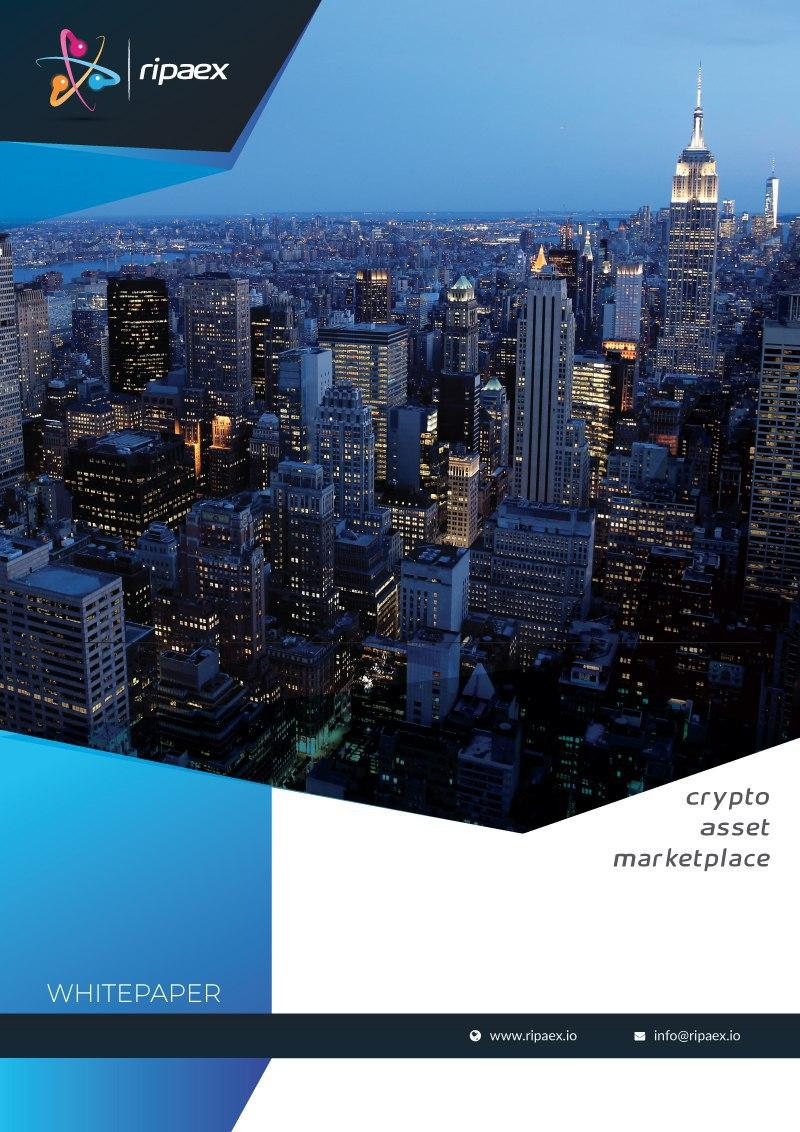
\includegraphics[height=\paperheight]{background}};
\end{tikzpicture}
\endgroup

\newpage

% \begingroup
% \section{Abstract}\index{Abstract}
% \thispagestyle{empty}
% \addcontentsline{toc}{chapter}{\textcolor{trolleygrey}{Abstract}}
\usechapterimagefalse % If you don't want to include a chapter image, use this to toggle images off - it can be enabled later with \usechapterimagetrue
\chapter{Abstract}
\textbf{Ripa Exchange is a hybrid-decentralized exchange with a strong focus on lowering the entry level
of opening new exchanges and giving crypto traders safe and secure trading partners to operate on a daily basis.}\\

The team of Ripa Exchange believes that, despite the recent developments in the world of
cryptocurrencies, it is still expensive to open, manage and build trust on a newly created exchange not
only for the resources need to run a reliable exchange platform but also for the build of the platform 
itself and to find the liquidity necessary to run a profitable business in the first 3-5 year gap.\\

Action is needed and action is needed now. Users are frustrated with unreliable exchanges that run away
with their funds, got hacked or does not sustain the load of a growing industry like this is. Despite
the effort of exchanges managers to offer efficient, reliable, and easy to use platforms to trade entry
prices for building such platforms is in the rage of five-six hundred thousand dollars and that does not 
include personnel cost to give platinum customer support, platform infrastructure and daily expenses for
the business. All of that for then having an decent exchange platform for which you will need to pay an 
external software company to make changes as you request.\\

It is the aim of this project to give you an Open Source, efficient, reliable exchange platform and to
give the needed liquidity\footnote{Thank you to the RLSP (Ripa Liquidity Service Provider) technology} to your newly created 
exchange from day \textbf{one} so you can focus on finding your customers, give platinum support and comply with all the heterogeneous 
laws in the industry. As we want that the customer experience will be the best (the sleekest) as possible while making them safer to trade.\\
\usechapterimagetrue
% \endgroup

%----------------------------------------------------------------------------------------
%	TABLE OF CONTENTS
%----------------------------------------------------------------------------------------

%\usechapterimagefalse % If you don't want to include a chapter image, use this to toggle images off - it can be enabled later with \usechapterimagetrue

\chapterimage{chapter_head_1_Beijing.jpg} % Table of contents heading image
% \addcontentsline{toc}{chapter}{\textcolor{trolleygrey}{Table of Contents}}
\renewcommand*\contentsname{Table of Contents}
\tableofcontents % Print the table of contents itself

% \pagestyle{empty} % No headers

% \cleardoublepage % Forces the first chapter to start on an odd page so it's on the right

% \pagestyle{fancy} % Print headers again

%----------------------------------------------------------------------------------------
%	PART
%----------------------------------------------------------------------------------------


%\part{Part One}

%----------------------------------------------------------------------------------------
%	CHAPTER 2: Introduction
%----------------------------------------------------------------------------------------

\chapterimage{chapter_head_2_London.jpg} % Chapter heading image

\chapter{Introduction}
- The industry of virtual currencies has (a high entry level from a technical point of view for the average user
and) an high entry level from an economical point of view for the average entrepreneur for buying a reliable cryptocurrency 
exchange source code, to hire professional DevOps personnel, to hire customer support operatives, to comply with national and 
international AML/KYC regulations to have liquidity from day one of the exchanges operations. We want to lower this entry level because
\textbf{running an exchange is HARD} and we want you to focus on things that matters not of caveats that the industry require because
you want to start to make business in this industry and you need the source code to do it.

To strengthen that there is the point that starting an exchange require an high level of investments form your venture capital 
and also with that the profit of your exchanges operations are not guaranteed in the first 5 years timespan.

For building a professional exchange services we think that the source code of your exchange and the liquidity to offer to your clients
from day one should be given to you free of charge: no more paying \$150,000.00 to a company just to have a platform that works and for
which you need to pay another \$100,000.00 - 150,000.00 just to brand it and customize as for your needs so you can tide your 
business to a company that may go bankrupt in the future and found you in trouble as you never had the source code of the product
your business rely on.

\textbf{We believe that all of this should be free} and we should offer you the best technology in the market so you can focus on your business
while we focus on building the technology to run your business in an efficient, secure, responsive and productive way. That is why Ripa Exchange 
is focusing on building a network of exchanges focusing on an exchange architecture that is \textit{efficient, secure, UI responsive, compliant and customizable}
so each exchange in the network can rely on solid foundations while customising its single exchange instance for the needs 
the business entity of that particular exchange installation needs is easy to you/accessible to you.

For reaching that goal we chosen to build our Ripa Liquidity Service Provider technology on top of ARK - a blockchain for consumer adoption - 
which primary focus is increasing consumer adoption for blockchain technologies focusing on two critical areas: \underline{A Fast Secure Core Technology}
and \underline{Practical Services for Real People}. ARK ecosystem is still at its early stage of development: in current implementation 
there is the possibility to run smart contracts natively on the ARK 2.0 blockchain, this will permits this blockchain technology to compete 
with Ethereum from a technological point of view. RLSP will permits to share the same liquidity-orderbook to each exchange in the Ripa Network based on
single exchange installation privacy rules, preferences in the admin area of your single exchange instance.

The Ripa Founder Team (RFT), as presented on ripaex.io, acts in the name of the Ripa Crew. The RFT is responsible for the proper use of 
funds collected under the Token Exchange Campaign (RIPA - TEC) presented below in this document.

The RFT undertakes that the result of this TEC will be used exclusively for the financing of the \emph{Ripa Exchange} project as explained in this 
whitepaper - which will be made available on the collection platform: tec.ripaex.io - and which should result in the creation of a 
legal entity whose name will be \emph{Ripa Exchange}. The creation of this company is scheduled for the first quarter of 2019.

To this end, RFT intervenes on behalf of \emph{Ripa Exchange, a company in the process of being incorporated}.


%------------------------------------------------

%This statement requires citation \cite{article_key}; this one is more specific \cite[162]{book_key}.

%------------------------------------------------

\section{Key Terminology}
\begin{description}
	\item[\textsc{Ripa Exchange:}] a FIAT <-> CRYPTO exchange (a cryptocurrency exchange) based on the source code
	of Peatio \cite{peatio}
	\item[\textsc{Ripa Blockchain:}] a DPOS blockchain in which liquidity is exchanged for all the exchanges in the Ripa network
	\item[\textsc{Ripa Token - XPX:}] a cryptographically secure token exchanged on the Ripa blockchain based on the DPOS protocol
	\item[\textsc{RIPA:}] the DPOS financial ecosystem composed of Ripa Exchange and Ripa Blockchain
	\item[\textsc{RIPAEX:}] the name of the project, project website and hosted domain
    \item[\textsc{RLSP:}] Ripa Liquidity Service Provider, a shared orderbook to exchange orders between exchanges in the same Ripa network
	\item[\textsc{RipaEx ICO:}] the name of fixed exchange rate token exchange period composed of both the phases of presale and RIPA TEC
	\item[\textsc{ARK:}] a platform for consumer adoption of blockchain technologies \cite{ark}
	\item[\textsc{ACES:}] Ark Contract Execution Services \cite{aces} provides simple protocols and tools for building a robust 
	blockchain service marketplace based on the ARK SmartBridge technology
    \item[\textsc{“,” or “.”:}] The Anglo-Saxon use of decimal points and commas to represent numbers has
been chosen for the purposes of this document: that is to say that a “.” represents a decimal point, and a “,”
distinguishes between multiples of thousands, millions and billions.
    \end{description}

%Lists are useful to present information in a concise and/or ordered way\footnote{Footnote example...}.
\pagebreak
\section{Roadmap}
There are essentially four phases to the RipaEx project:\\

\tcbset{roadmapBox/.style={colback=yellow!10!white,colframe=azure(colorwheel),
equal height group=nobefaf,width=(\linewidth-1pt), height from=4cm to 8cm, nobeforeafter,
	center title,
	valign=top, halign=left}}
\begin{center}
\begin{tcolorbox}[roadmapBox,
	title=\textbf{\textsc{Funding the project: XPX presale and RIPA TEC (WP2)}}]

	This phase recognises the existence of interest in this market development
	from across the World concerning the lowering of the entry level for building a cryptocurrency exchange.
	It aims to make the first comprehensive analysis of this state of the art to form the basis of the later project phases and
	build the first working prototype of a centralized exchange based on Peatio.\\
	\vspace{1cm}
	\centering\textbf{\textsc{Phase ending December 2018}}.
\end{tcolorbox}

\resizebox{0.05\textwidth}{26pt}{$\Downarrow$}

\begin{tcolorbox}[roadmapBox,
	title=\textbf{\textsc{First exchange opening and development of tools and resources (WP3)}}]

	The second phase takes the results of the first 
	and develops from them a set of tools and resources which provide concise and comprehensible guidance to market actors in any
	Country. With the first instance of Ripa Exchange running first contacts with other economical players in the industry can be
	done.\\
	\vspace{1cm}
	\centering\textbf{\textsc{Phase ending June 2019}}.
\end{tcolorbox}

\resizebox{0.05\textwidth}{26pt}{$\Downarrow$}

\begin{tcolorbox}[roadmapBox,
	title=\textbf{\textsc{Dissemination (WP 7/8) and Project Coordination (WP1)}}]

	During the full duration of the project, 
	dissemination activities (WP 7/8) are carried out in which results from the individual work packages are disseminated 
	to relevant target groups including project partners, RipaEx supporters, exchanges managers, banking partners as well 
	as relevant target groups. This phase covers a wide range of dissemination techniques, from printed and
    electronic handbooks to workshops and training sessions, ongoing networks, all having the
	ultimate goal of defining a standard for exchanges communication among public and private entities. 
	An overarching work package is concerned with the management of the project from start to finish, ensuring proper coordination, 
	quality assurance and budgetary control (WP1).
\end{tcolorbox}

\resizebox{0.05\textwidth}{26pt}{$\Downarrow$}

\begin{tcolorbox}[roadmapBox,
	title=\textbf{\textsc{Development of hybrid-decentralized exchange (WP 4-6)}}]

	Using the tools and resources developed in WP3, 
	Work packages 4-6 focus on bringing collected knowledge and tools into practice. The three work packages reflect three major
	focal points (and target groups) within the network of exchange created for establishing successful 
	demonstrations on local scale: incorporations of local Ripa Exchanges (WP4), technical analysis for the 
	Ripa Liquidity Service Provider (WP5), and first MVP of the hybrid decentralized exchange (WP6). The demonstration
    phase forms the heart of the RipaEx action; WP 2 and 3 are focused on providing
	deliverables (e.g. tools) that enable successful and efficient demonstration activities.\\
	\vspace{1cm}
	\centering\textbf{\textsc{Phase ending January 2021}}.
\end{tcolorbox}
\end{center}

\section{RipaEx Partners - RipaEx Governance}\index{RipaEx Partners - RipaEx Governance}
Most of the partners are entrepreneurs in the virtual currency industry, but a research institute 
and Financial Organizations are also represented. The Partners are:
\begin{description}
	\item[Coordinator]: Ripa Exchanges Ltd
	\item[CoBeneficiaries]: 
\end{description}
\subsection{RipaEx Governance}\index{RipaEx Governance}
Governance for the network of exchanges created, development of the source code, owning of the XPX tokens, Ripa Foundation.

\section{Project Summary}
\begin{enumerate}
	\item \textsc{what}: RipaEx is a project to facilitate the uptake of standards to share liquidity between crypto assets marketplaces. 
	The objective of RipaEx is the promotion of shared source code for wallets and exchanges in the virtual currency industry: 
	It is the aim of this reference document to give in-depth information to prospective exchange developers,
	or exchange managers, to enable correct decision-making and to ensure success for their proposed projects. 
	It seeks to analyse the real potential in the Country of application for a network of cryptocurrency exchanges, 
	and its place in the market.
	\item \textsc{what}: Crypto assets are an alternative to centralized assets managed by (country-specific) stock exchanges. Although certain
	stock exchanges gives the possibility to their users to verify and manage the assets they own the verification process
	is not always transparent that is the reason because from 2009 \cite{bitcoin} onwards a new types of (community-verifiable) assets 
	have been implemented to give small, medium and big investors complete transparency in the managing of their investments
	assets.
	\item \textsc{when}: Recent developments at European Union level and worldwide are transforming both how virtual currencies
	are treated and the way ICO (Initial Coin Offering) are legislated. These combined developments 
	have made the use and production of virtual currencies an increasingly favourable prospect. \\
	In October 2015 the European Court of Justice ruled that bitcoin and other cryptocurrencies are exempt from VAT taxation. \\
	In July 2016 the European Commission adopted proposals for legislation to amend the 4th Anti-Money Laundering Directive (4AMLD) that
	will bring virtual currencies exchanged and wallet providers into the EU's anti-money laundering framework \cite{EUAMLCrypto}.\\
	In February 2018 the European Commission launched the EU Blockchain Observatory and Forum \cite{EUBOaF} to highlight key developments 
	of the blockchain technology, promote European actors and reinforce European engagement with multiple stakeholders involved in blockchain activities.
	\item \textsc{why}: However there is still very little regulation performed on ICOs and only United States of America at the moment has undergone
	a legislation defining ICO tokens as securities. \cite{SECICO}
	\item \textsc{who}: The results indicate that medium tech savvy from 18 to 45 is the average user of
	virtual currencies although the corporate finance companies are also starting to put 
	virtual currencies schemes inside their portfolio especially since the presentation 
	of the bitcoin futures contract from CME Group Inc. in the stock exchange of Chicago
	last 18th of December 2017.
	\item \textsc{how much}: Total virtual currencies market capitalization has been estimated around 317 B USD\footnote{Coinmarketcap data April 2018}
	and is predicted to grow to 5,000.00 B USD in the next ten years span \cite{cryptoMCTenYears}.
	\item \textsc{where}: Local authorities are working with National Governments to make sure local exchangers
	in the national territory are complying with national and international AML/KYC regulations.
	Venture capitals and Angel Investors are starting to release financing solutions to start-ups 
	in the Fintech industry all over the world from America to Asia passing through Europe and some 
	Countries are starting state-owned cryptocurrencies schemes to test the exchange of goods \& services
	on those (distributed ledger) technologies \cite{petro}.
	\item \textsc{how much}: The average cost for starting your own crypto asses marketplace is around \$ 150,000.00 only for a running instance of your exchange platform:
	to that you need to add costs to customize the platform before launch and in the future, advertising your new business, running costs for servers,
	network operators, support center operators and legal department to comply with your State of incorporation AML/KYC legislations and general company laws.\\
	\textbf{That is the reason because we think owning the source code of your exchange software is the best way to run a business in this industry}.
	\item \textsc{how}: The main problems encountered in opening a FIAT <-> CRYPTO marketplace is to find trusted
	banking partners to comply with the many different AML/KYC rule and procedures to exchange virtual currencies
	to FIAT currencies.
	\item \textsc{what}: Classical types of exchanges operations are: 
		\begin{enumerate}[label*=\arabic*.]
			\item \textbf{one-way exchanges}: in which a centralized application has all the liquidity to offer to its potential users
			\item \textbf{two-way exchanges}: in which a centralized or decentralized platform match the selling requests with the buying requests
			of its users
		\end{enumerate}
		On this a sub-classification is also necessary:
		\begin{enumerate}[label*=\arabic*.]
			\item \textbf{FIAT <-> CRYPTO exchanges}: in which exchanges operations are performed between FIAT\footnote{Traditional central banks owned currencies like EUR, USD, GBP, JPY, others...} 
			currencies and virtual currencies
			\item \textbf{CRYPTO <-> CRYPTO exchanges}: in which exchanges operations are performed only between virtual currencies
		\end{enumerate}
	You can build a matrix based on the four configurations above to build the exchange operation platform of your needs.
	\item \textsc{with what}: The specifications to look when choosing for an exchange platform to run are:
		\begin{enumerate}[label*=\arabic*.]
			\item \textbf{code}: Open Source, Closed Source or hybrid solution
			\item \textbf{modularization}: separation between exchange engine (orders matching engine), UI and user registry
			\item \textbf{UI responsiveness}: responsiveness of UI on all devices (desktop and mobile)
			\item \textbf{compliance}: with current industry standards
			\item \textbf{customization}: of the exchange engine, trading currencies, UI and other aspects of the crypto asset marketplace platform...
			\item \textbf{security} of the funds: saving in cold wallets and hot wallets configurable
			\item \textbf{transparency} of the funds: proof of solvency of the exchange
			\item \textbf{Multi-Accounts trading}: easy to configure new virtual currency protocols
			\item \textbf{Multi-Accounts users}: possibility to interact with user accounts from Google, Facebook, Twitter 
			to login into the platform and FIDO Alliance security standards for personal credentials.
		\end{enumerate}	
	\textbf{Those are not only technical decisions to be made but also economical} especially the owning of the source code of your crypto asset
	marketplace platform is fundamental to make future customization of your exchange in an independent way compared to rely on a single
	software house that makes the customizations for you.
	\item \textsc{how}: Options for finding users for your exchanges operations are: targeted marketing campaigns, innovative features in the industry,
	fee level based on trading quantities, bonuses for first registration and trading quantities, affiliate marketing for paying users to take their friends
	to your exchange.
	\item \textsc{how}: For setting-up a crypto asset marketplace a project must take into account the following legislation:
		\begin{enumerate}[label*=\arabic*.]
			\item \textbf{AML/KYC}: \textit{Fourth Anti-Money Laundering Directive} if business set up in the European Union \cite{4AMLD} or the AML/KYC reference implementation
			to your crypto asset marketplace Country of incorporation (as an example \textit{Intelligence Reform \& Terrorism Prevention Act of 2004}
			written by FinCEN in the United States of America).\\
			International recommendations for undergoing AML/CFT verifications are given by the Financial Action Task Force on Money Laundering \cite{FATF}.
			\item \textbf{Payment Licence}: By far the biggest and most arduous task with regards to legitimising the 
			FIAT <-> CRYPTO exchanges operations is obtaining a \textit{PSD Licence} \cite{PSD}. 
			The PSD licence follows Council Directive 2007/64/EC and is applied in each country via its own national laws. 
			Costs of an PSD licence can vary between \euro XXXX and \euro XXXX, depending on the exchange volume.
		\end{enumerate}
	\item \textsc{who}: The nature of the business under consideration by the Ripa Exchange project (small scale,
	localised FIAT <-> CRYPTO exchanges operations), means that each enterprise likely to have 7 or 8 staff: N.2 developers, 
	N.1 network/security operator, N.1 administrative, N.2 client support operators, N.1 legal and tax advisor. \\
	The turnover of such an enterprise however, because of the high value of the end product, is likely to be more than 
	\euro 350,000 a year and could be several times higher. A business of
	this scale lends itself to the following possible company structures: A simple partnership;
	A limited company; A non-profit company or social enterprise; A worker co-operative.
	Financial Agencies are potential key actors, but the type of business they can set up will
	depend on their legal status which does vary from country to country.
	\item \textsc{how}: Potential sources of funds for a small-medium sized crypto asset marketplaces are: Bank Loans; Low
	Interest Loan Schemes; Commercial Credit; Equity financing; Business Angels venture
	capital. Having a robust Business Plan and financial guarantees are essential elements
	for securing funding. The European Investment Fund (EIF) of the EIB, offers support in
	the form of guarantees for SMEs.
	\item \textsc{why}: The arguments for crypto asset marketplaces are for financial freedom, decentralizing of the value-transferring operations, and
	owning for real your money. 
	There are other benefits, well documented, such as faster payments, long term gain based on deflationary economy and prediction of 
	Great Depressions like the one that hit the global economy in 2008. But
	above all, virtual currencies are the only direct competitor to centralized value-transferring operations done by central banks.

	\item \textsc{why}: There is consensus in the literature that the use of virtual currencies in place of fiat currencies will result in 
	higher financial freedom especially as they fit into the Austrian school of economy \cite{austrianTheory} 
	(TODO: add more on Austrian economics school)

	\item \textsc{why}: Benefits of virtual currencies schemes (TODO: put some numbers)

	\item \textsc{how}: Securing assets on the blockchains means basically performing three operations
		\begin{enumerate}[label*=\arabic*.]
			\item \textbf{Generating a random private key}
			\item \textbf{Converting the private key generated in (1) into a public key}: a common protocol making this conversion
			in the virtual currencies industry is the ECDSA curve algorithm
			\item \textbf{Converting the public key generated in (2) into a virtual currency address}: common protocols for making this conversion
			are hash functions SHA-256, Base58 encoding, Base32 encoding
		\end{enumerate}
	At this point any value sent to the virtual currency address generated in (3) is secured on the blockchain of choice and accessible
	only from the owner of the relative private key generated in (1).
	\item \textsc{where}: The two critical factors affecting the cryptocurrency industry are banks concurrence and State banning.
	Although a harmonisation throughout Europe would be beneficial to development of the industry both in terms of 
	taxation and warranty approvals, this is currently not the case. Each country has its specific legislation and tax
	regime for all exchanges operations involving FIAT money, and State banning is going to completely liberalization 
	of this activities like European Union to complete banning and imprisonment of operators in this industry like Bangladesh
	\cite{bitcoinLegality}. 

	\item \textsc{where}: The Asiatic countries of South Korea, China and Japan are the leader in the field of cryptocurrencies for number of 
	transactions for over 9 years with a proactive approach and favourable tax regime. At the beginning of 2017 in Japan bitcoin
	has been declared legal tender but China has recently declared illegal token sale and exchanges and local cryptocurrencies
	marketplaces are closing down.
	\item \textsc{where}: Any assessment of your local market should include: number of potential users to reach, 
	type of exchange to incorporate (FIAT <-> CRYTPO or CRYPTO <-> CRYPTO), type of virtual currencies protocol 
	to integrate (POW, DPOS, Masternodes, others...), types of services to offer (exchange only, advanced trading tools,
	payment processor, others...), if FIAT <-> CRYPTO exchange number of FIAT payments processors to accept (PayPal, OKPay,
	MoneyPolo, others...), number of others exchanges in your region.

	\item \textsc{who}: there are a number of options for dealing with Warranty/Customer protection issues: 
	creating consumer pressure by making clear to the end users that the possession of the private keys of their
	virtual currency addresses make \textbf{liable} for any loss of the private keys meaning nobody can help
	them recovering their funds if the their private keys are lost. Creating consumer pressure to not leave funds
	on exchanges ("\textit{Be Your own Bank!!}"), making them choose the licensed exchanges in the market. 
	\item \textsc{who}: While it is very expensive to insure money exchanges operations and money transmitting operations, 
	examples of customer protections in the industry are: Kraken platform which is offering Mt. Gox users partial refund
	of their lost, NEO community giving refund to the users involved in the BitGrail hacking, Ethereum supporters
	giving The DAO investors partial refunds, other hacking cases...

	\item \textsc{Recommendations for all/law compliance}: if you intend to incorporate a FIAT <-> CRYPTO exchange you should
	focus from the first instance on law compliance by studying the AML/KYC laws of the country of incorporation and
	finding bank partners to work with. Local financial Authority can help to comply with rules \& regulations and 
	local cryptocurrencies foundations can help you to tune your exchanges operations to perform targeted
	operations based on the customers interests in the country of incorporation.
	Promote cryptocurrency-friendly users in the area of interest.
\end{enumerate}


%----------------------------------------------------------------------------------------
%	CHAPTER 3: Ripa Exchange
%----------------------------------------------------------------------------------------

\chapterimage{chapter_head_3_Singapore.jpg} % Chapter heading image

\chapter{The Ripa Exchange}
Ripa Exchange is an crypto asset (fiat money or cryptocurrency or something) marketplace, following the latest 
industry standards and resting in the principles of "\textit{open source, secure and efficient}". Ripa Exchange
aims to serve a platform for crypto-currency enthusiasts by providing a safe, secure, UI responsive, customizable 
and easy to use exchange that embraces open source principles and public trust.\\\\
Ripa Exchange is implemented with the Rails framework and other cutting-edge technology and will be migrated to an
hybrid-decentralized exchange where all exchanges in the Ripa network will share liquidity thanks to the RLSP technology.

\section{Mission}
\begin{quotation}
	``\textit{Our mission is to build the world best open source crypto asset marketplace with a high performance trading engine 
	and safety which can be trusted and enjoyed by users. Additionally we want to move the crypto currency exchange technology 
	forward by providing support and add new features. We are helping people to build easy their own exchange around the world.}''
\end{quotation}

Help is greatly appreciated, feel free to submit pull-requests or open issues.

\section{Features}
A free, transparent and internationalized open source crypto currency exchange.\\

\tcbset{featureBox/.style={colback=yellow!10!white,colframe=white!20!black,
equal height group=nobefaf,width=(\linewidth-1pt)/3, height=4.5cm, nobeforeafter,
	center title,
	valign=top, halign=left}}
\begin{tcolorbox}[featureBox,
	title=\textsc{Open Source}]

	\small	All source code are fully released under the terms of the MIT License.\\\vspace{5mm}
	\tiny Ripa Exchange is a customizable cryptocurrency exchange solution architecture enables easy connection to KYC/AML, 
	authentication, ETL/reporting, and other services.
\end{tcolorbox}
\begin{tcolorbox}[featureBox,
	title=\textsc{Compliant}]

	\small	International KYC/AML standards.\\\vspace{5mm}
	\tiny Ripa Exchange KYC efficiently submits and exchanges KYC information 
	to meet the banking supervisory standards and comply with Customer Due Diligence (CDD) requirements.
\end{tcolorbox}
\begin{tcolorbox}[featureBox,
	title=\textsc{Transparent \& Configurable}]

	\small	Customize in your own way\\\vspace{5mm}
	\tiny Major functions have been embedded in the source code – neat registration and log-in interface, 
	personalized deposit and withdraw procedure, best match of bid and ask, etc. These functions are comprehensive 
	and are ready to use with no extra work needed. 
\end{tcolorbox}

\begin{tcolorbox}[featureBox,
	title=\textsc{Internationalization}]

	\small	All users are able to view Ripa Exchange in a language to their best convenience.\\\vspace{5mm}
	\tiny Supporting many common languages, Ripa Exchange makes it easy for users to operate in their mother tongue. 
	You are encouraged to contribute to our language variety. Users will benefit from your efforts.
\end{tcolorbox}
\begin{tcolorbox}[featureBox,
	title=\textsc{Proof of Solvency}]

	\small	Easy deployable PoS.\\\vspace{5mm}
	\tiny Ripa Exchange Proof of Solvency (PoS) allows users to verify 
	the solvency of the Ripa Exchange based cryptocurrency exchange without compromising user privacy.
\end{tcolorbox}
\begin{tcolorbox}[featureBox,
	title=\textsc{Multi-Accounts Trading}]

	\small	Easy currency configuration.\\\vspace{5mm}
	\tiny Ripa Exchange allows to create multiple accounts and trading in multiple currencies. 
	Ripa Exchange makes it is easy to trade different currencies.
\end{tcolorbox}

\begin{tcolorbox}[featureBox,
	title=\textsc{Multi-Accounts Users}]

	\small	Easy account configuration.\\\vspace{5mm}
	\tiny Ripa Exchange allows to create multiple login accounts Google, Facebook, Twitter and FIDO Alliance
	login standards to secure your account.
\end{tcolorbox}
\begin{tcolorbox}[featureBox,
	title=\textsc{Enterprise Exchange}]

	\small	Start small, grow big.\\\vspace{5mm}
	\tiny Ripa Exchange enterprise exchange features include a high-performance matching engine, 
	scalable distributed worker threads, and SMS 2-factor authentication.
\end{tcolorbox}
\begin{tcolorbox}[featureBox,
	title=\textsc{Functional \& Intuitive}]

	\small	For the new trader, for the experienced trader.\\\vspace{5mm}
	\tiny Clean, user friendly registration and login interface. 
	Personalized deposit and withdraw procedure and a built-in proof-of-solvency audit.
\end{tcolorbox}

\section{Functional Analysis}
\begin{enumerate}
	\item \textsc{Why Redis-RabbitMQ is needed}:
	\item \textsc{Why NodeJS}: 
	\item \textsc{Why Pusher}:
	\item \textsc{ER MySQL}:
	\item \textsc{Ruby folders hierarchy}:
\end{enumerate}

\section{Technology Stack}
\begin{description}
	\item[\textsc{Ruby on Rails}]:
	\item[\textsc{MySQL}]: 
	\item[\textsc{Redis}]:
	\item[\textsc{RabbitMQ}]:
	\item[\textsc{NodeJS}]:
	\item[\textsc{Pusher}]:
\end{description}

\section{User Interface}
Ripa Exchange user interface is based on Peatio user interface a UI responsive user interface built in Ruby on Rails and 
completely separated from the exchange order engine.
Design for a customised UI are in place to offer to Ripa Exchange users the best experience on all devices: here you can find
some screenshot of the current exchange interface design.

\subsection{End-User Interface}
Following some screenshot of the end-user Ripa Exchange-Peatio interface: 
\textcolor{darkred}{those screenshots are a work in progress and they may not represents the user interface of the final product}\\
\begin{center}
	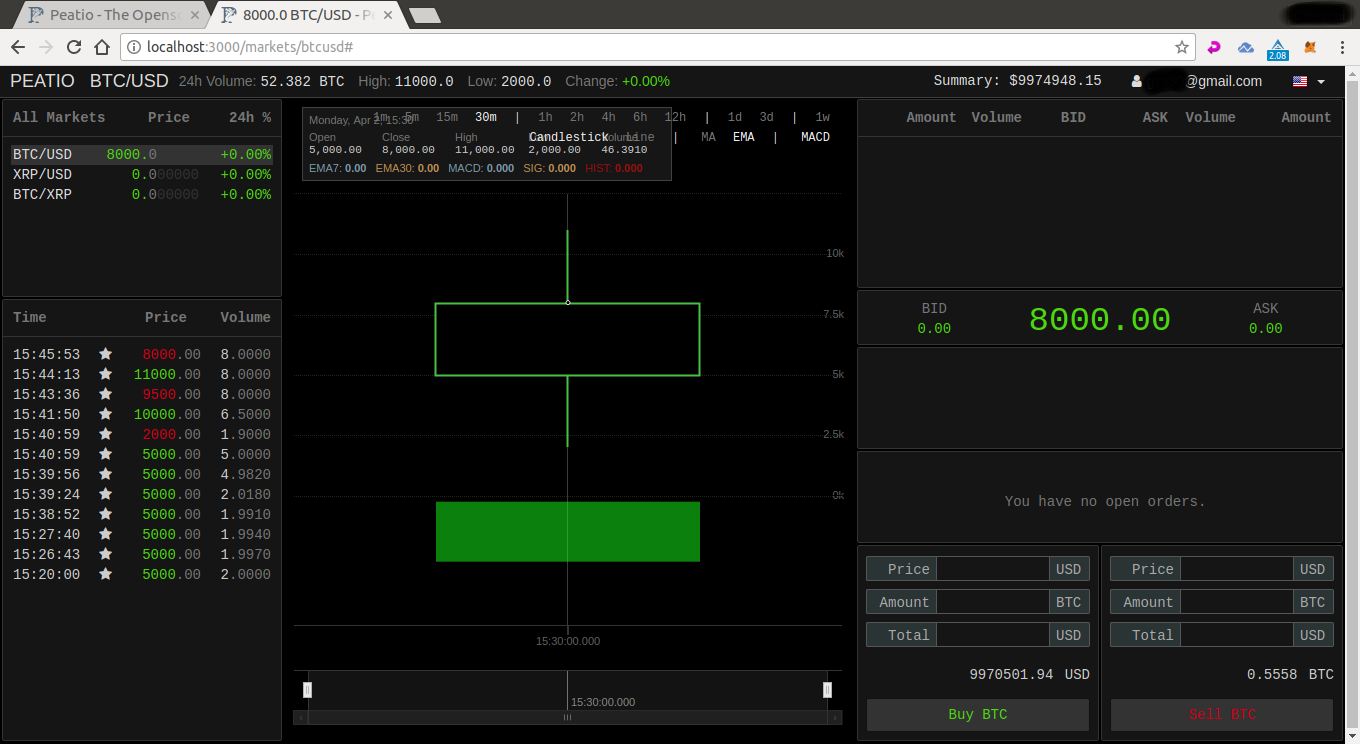
\includegraphics[width=\textwidth*2/3,height=\textheight,keepaspectratio]{RE_TradingUIC}
	\captionof{figure}{Ripa Exchange trading UI}
	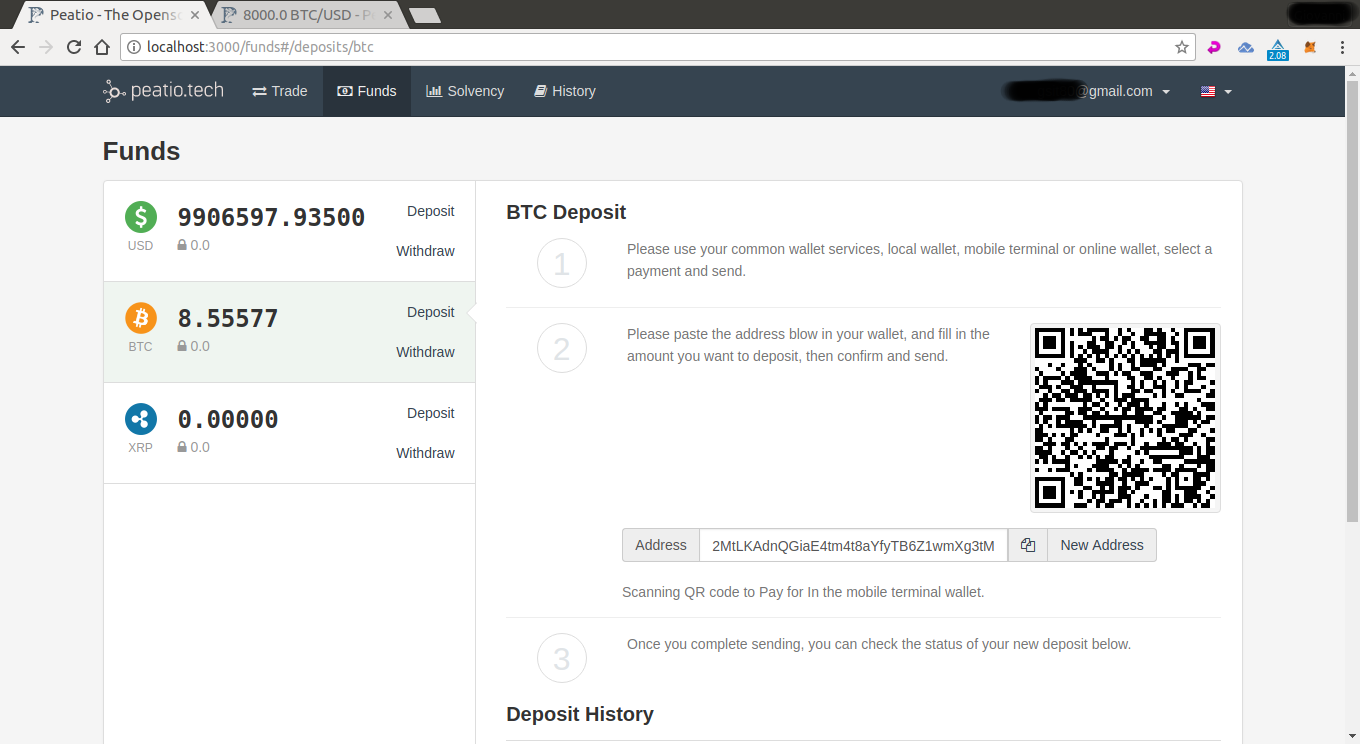
\includegraphics[width=\textwidth*2/3,height=\textheight,keepaspectratio]{RE_depositBTCC}
	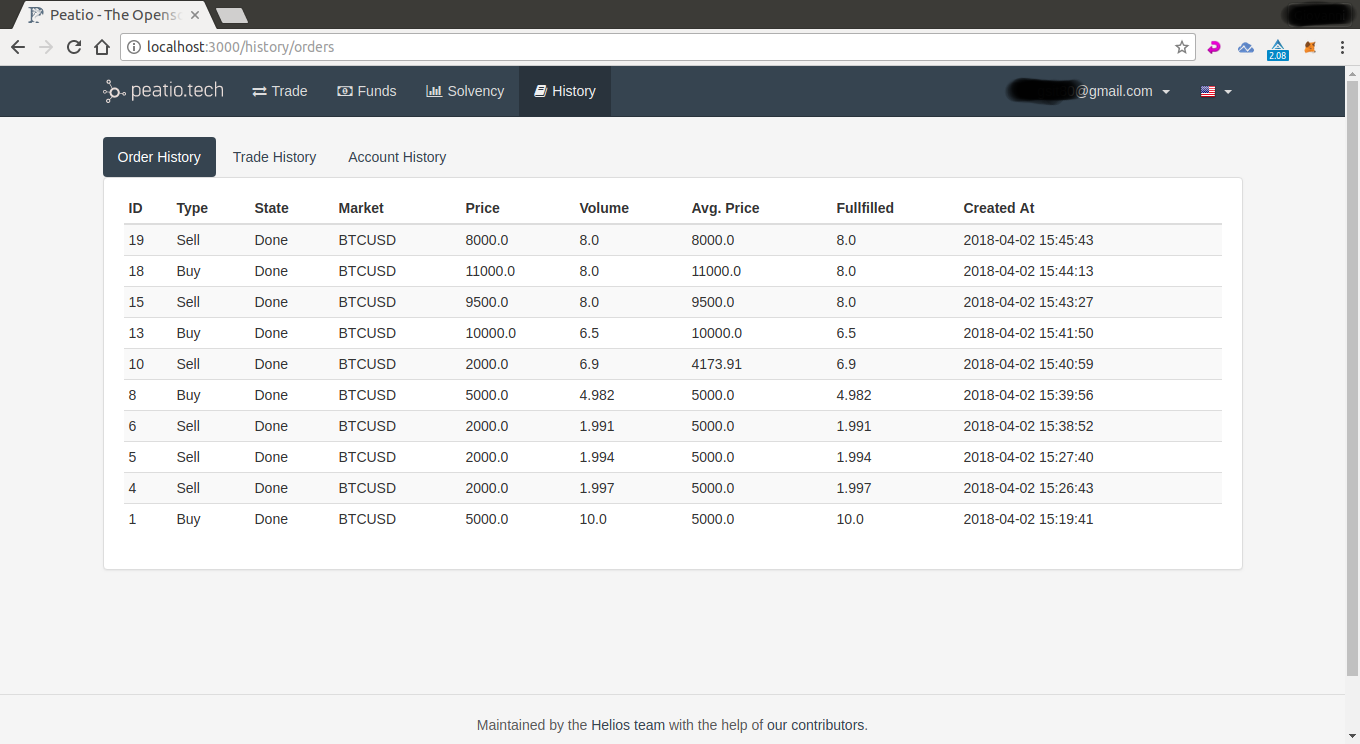
\includegraphics[width=\textwidth*2/3,height=\textheight,keepaspectratio]{RE_historyC}
	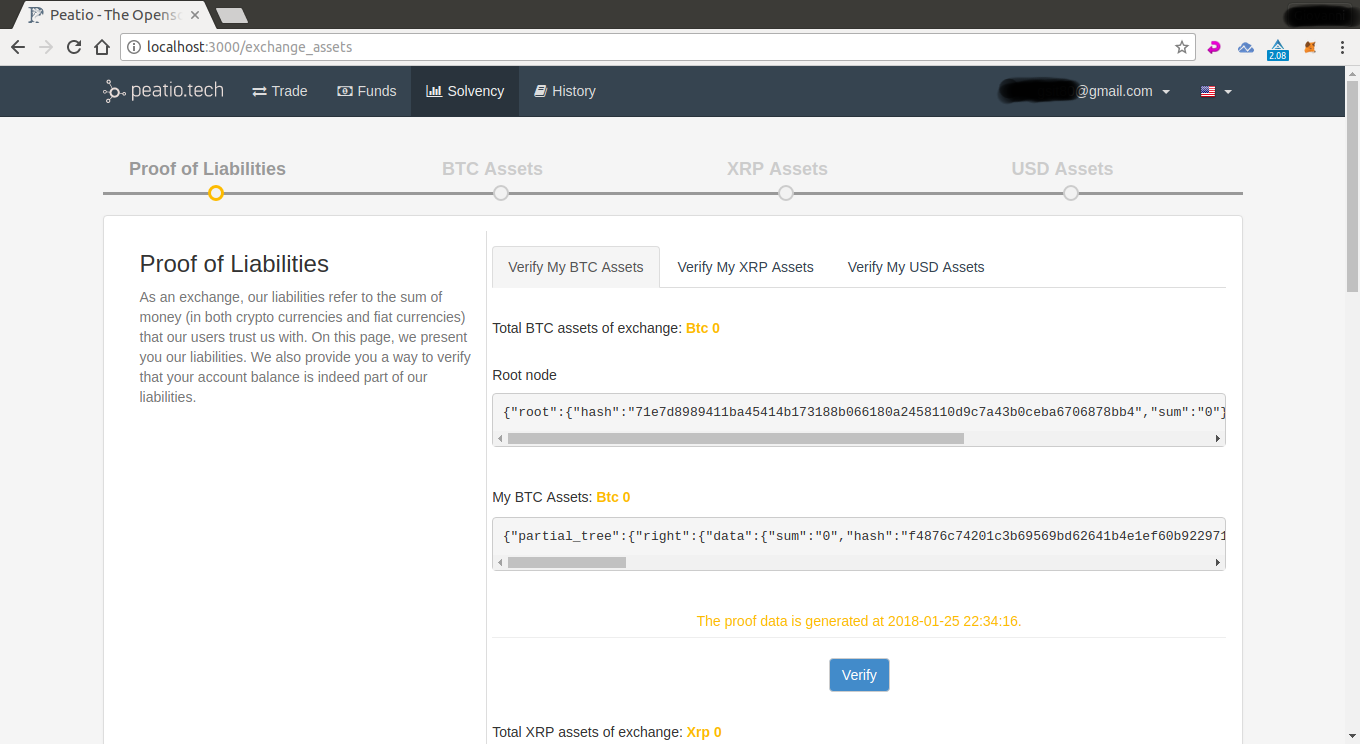
\includegraphics[width=\textwidth*2/3,height=\textheight,keepaspectratio]{RE_solvencyC}
	\captionof{figure}{Ripa Exchange deposit/whitdraw, order history and solvency screen}
\end{center}

\subsection{Admin Interface}
Following some screenshot of the administrative console of Ripa Exchange-Peatio interface: 
\textcolor{darkred}{those screenshots are a work in progress and they may not rapresents the user interface of the final product}\\
\begin{center}
	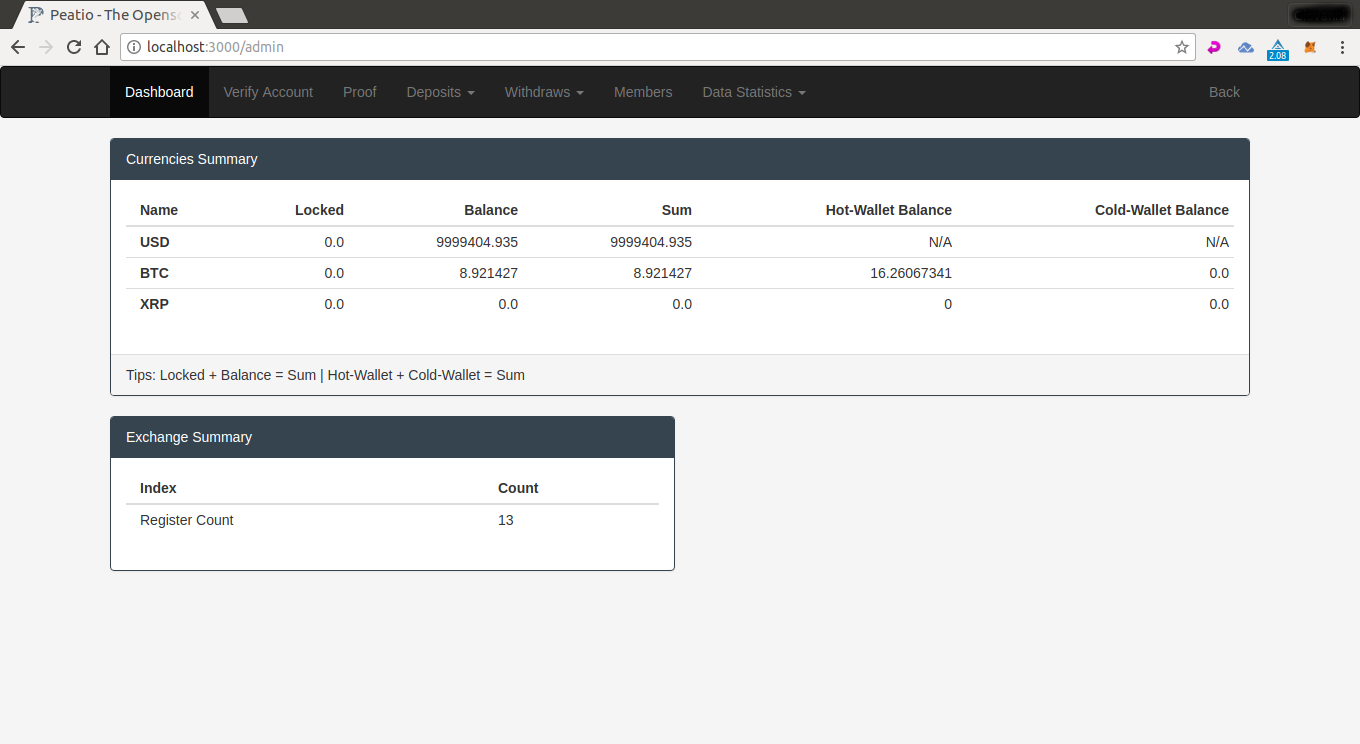
\includegraphics[width=\textwidth*2/3,height=\textheight,keepaspectratio]{RE_adminDashboardC}
	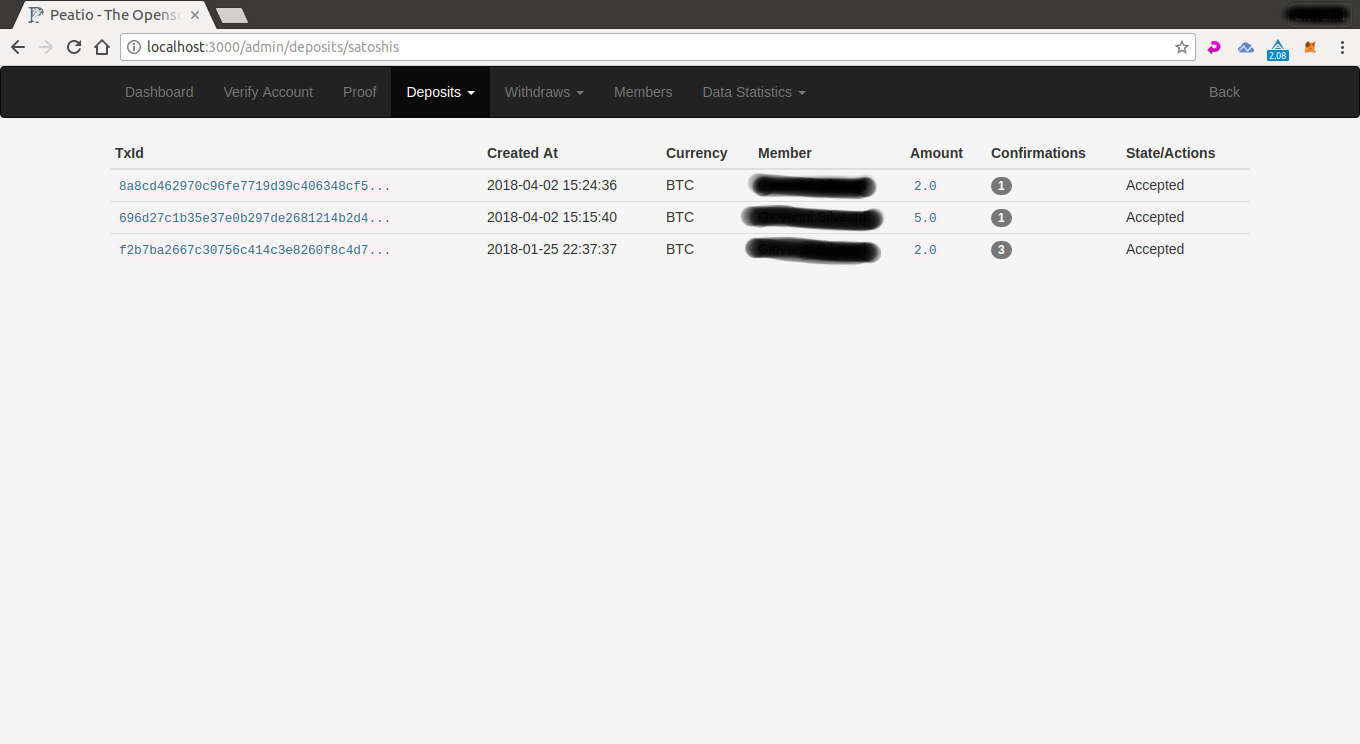
\includegraphics[width=\textwidth*2/3,height=\textheight,keepaspectratio]{RE_adminDepositsC}
	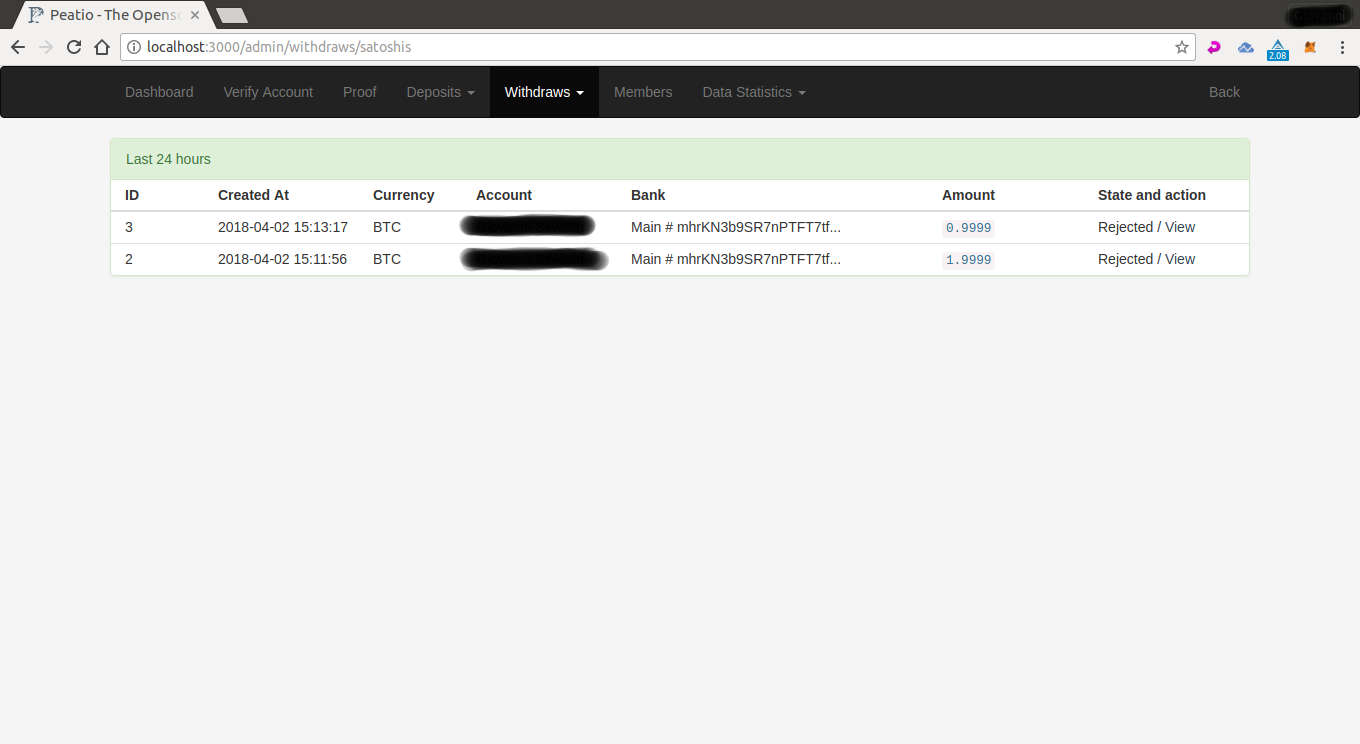
\includegraphics[width=\textwidth*2/3,height=\textheight,keepaspectratio]{RE_adminWithdrawsC}
	\captionof{figure}{Ripa Exchange Admin console dashboard, deposit/whitdraw screen}
	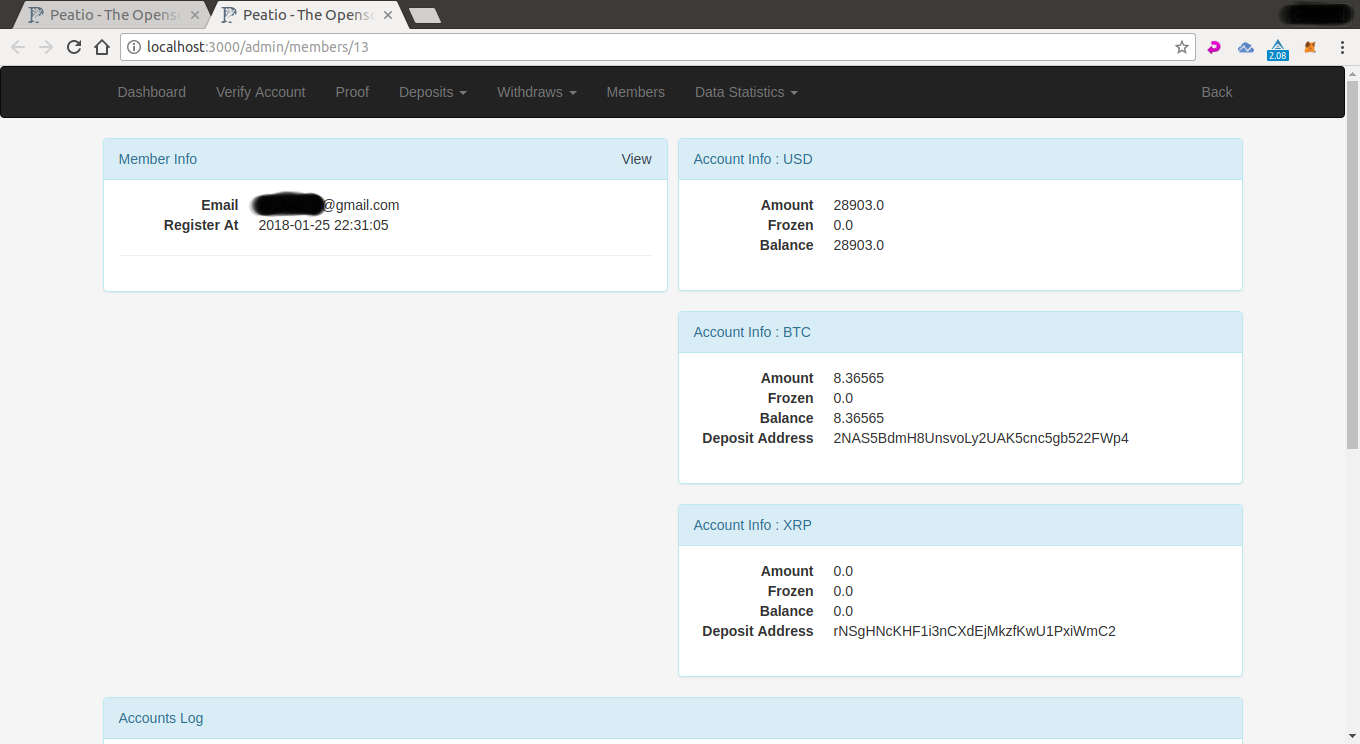
\includegraphics[width=\textwidth*2/3,height=\textheight,keepaspectratio]{RE_adminUserInfo1C}
	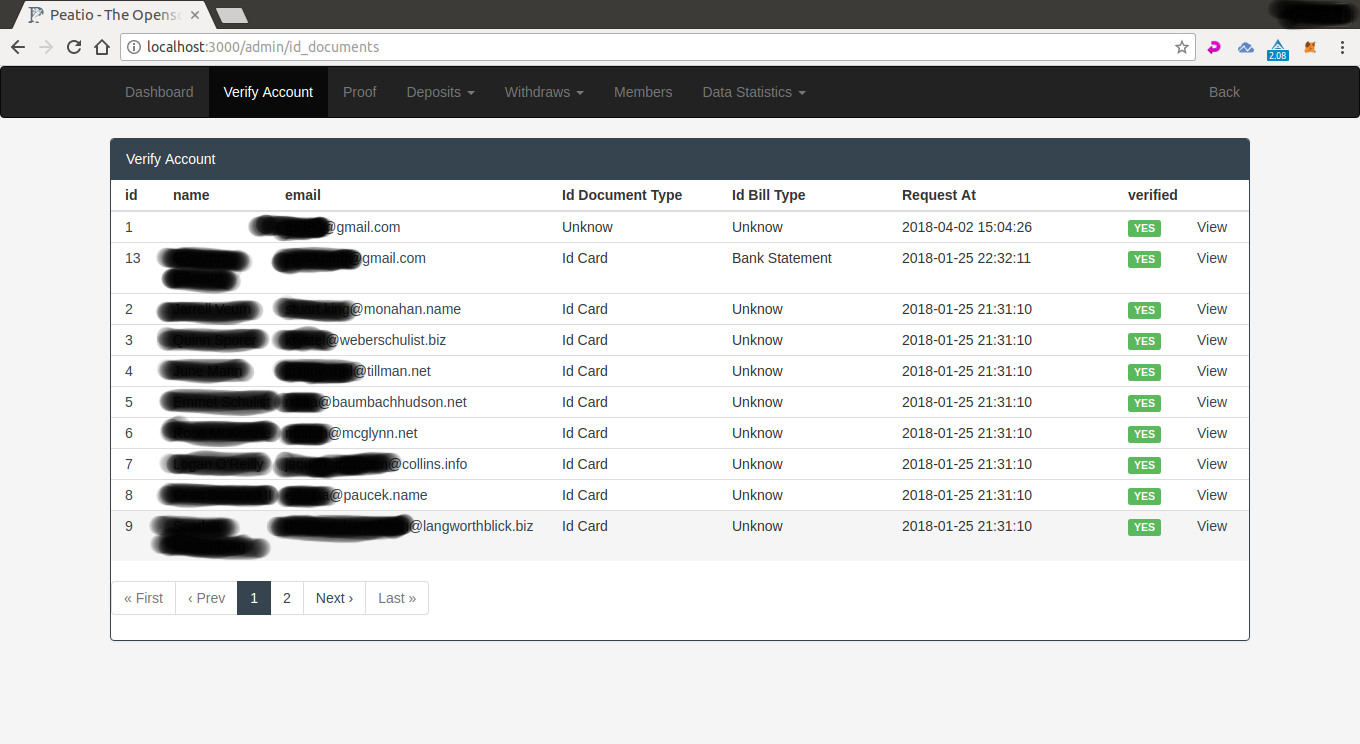
\includegraphics[width=\textwidth*2/3,height=\textheight,keepaspectratio]{RE_adminVerifyAccountC}
	\captionof{figure}{Ripa Exchange Admin user info and verify account screen}
\end{center}

\section{Features at Launch}
\begin{description}
	\item[\textsc{CRYPTO <-> CRYPTO}]:
	\item[\textsc{OAuth}]: Facebook, Google, Twitter
	\item[\textsc{FIDO}]: login with FIDO Alliance standards
	\item[\textsc{Protocols}]: POW, DPOS, Masternode, tether, ERC20
	\item[\textsc{Currencies}]: BTC, ETH, DOGE, BCH, TUSD, ARK, LISK, SHIFT, RISE, KAPU, OXY, RIPA, promising ERC20 tokens
	\item[\textsc{Main Markets}]: BTC, ETH, ARK
	\item[\textsc{Orders Type}]: market, limit
\end{description}

\subsection{Future Features}
\begin{description}
	\item[\textsc{E-Wallets}]: OKPay, NETELLER, MoneyPolo, others...
	\item[\textsc{Advanced Trading Features}]: margin trading, stop loss and take profit, 
	\item[\textsc{FIAT <-> CRYPTO}]
	\item[\textsc{Other tools}]: VISA/MasterCard, merchants tools, P2P Lending 
\end{description}


\section{Towards a Decentralized Exchange...}
Ripa Exchange is a centralized exchange which will be converted into an hybrid-decentralized exchange to create a network of exchanges
that share the same liquidity between each of them so you can offer liquidity from day 1 of your exchanges operations.\\

To offer the PROs of a centralized exchange with all the PROs of a decentralized exchange without the CONs of both of them, 
we need to convert first into an hybrid-decentralized exchange and during phase 3 of our project (WP4-6) we will make all the 
functional and technical analysis required to make the next step on solid ground.

%----------------------------------------------------------------------------------------
%	PART
%----------------------------------------------------------------------------------------

%\part{Part Two}

%----------------------------------------------------------------------------------------
%	CHAPTER 4: Ripa Blockchain
%----------------------------------------------------------------------------------------

\chapterimage{chapter_head_4_Dubai.jpg} % Chapter heading image
\chapter{The Ripa Blockchain}
The project RipaEx will have its own blockchain called Ripa which will be run on the DPOS protocol and has the \PHP 
token (XPX symbol) running on it that will serve the five following purposes:
	\begin{enumerate}
		\item to list new cryptocurrencies on Ripa Exchanges
		\item to advertise new projects
		\item to buy RipaEx gadget on Ripa Exchange Store
		\item to pay for the sell of goods \& services on authorized resellers with our RipaEx POS (Point of Sale)
		\item to share liquidity between Ripa Exchanges in the same network
	\end{enumerate}

Ripa \PHP or XPX is a cryptocurrency derivate from ARK, Lisk, Crypti and BitShares with unique differences and improvements
for reaching the goal of shared liquidity between exchanges in the same Ripa network. This code however inherits the 
simplified interactions between ARK and other blockchain systems using DPoS as their consensus. This homogeneous codebase
allows for the potential to provide service bridges in the form of ARK-Lisk blockchain apps, along with any other additional 
systems provided by their blockchain administrators.

\vspace{5mm}
\textsc{\textbf{Ripa blockchain is an ARK fork and the use of a blockchain technology for the network of exchanges created will complete
the ripa ecosystem by permitting each exchange in the ripa network to share the same liquidity. We will always entrust ARK as our 
blockchain technology provider to merge their code into our latest features for what concerning the RIPA Blockchain}}

\vspace{5mm}

Explained the use of the Ripa Blockchain in the RipaEx ecosystem and explained the RIPA - ARK technological relations what is 
following are the specifications of the Ripa Blockchain derived/inherited from ARK.

\section{Delegated Proof of Stake Technology}
Ripa Blockchain, will inherits the Delegated Proof of Stake (DPoS) consensus system that was first introduced
by BitShares. This consensus algorithm was designed to eliminate the issues associated with Proof of Work (PoW), 
namely the centralization of computing power and the exponentially increasing waste of real world energy. While not
completely decentralized as it relies on consensus by a fixed number of elected delegates, it guarantees a better decentralization 
than Bitcoin. The consensus algorithm implementation is improved over time, evolving into an optimal consensus system.\\

The technical description of the Ripa blockchain is as follow:
\begin{enumerate}
	\item DPoS (Delegated Proof of Stake)
	\begin{description}
		\item - 101 active forging Delegates
		\item - Delegates selected by vote mechanism built into DPoS
		\item - 115,000,000 RIPA - Seeded Genesis Block
	\end{description}
	\item Multi-signature accounts
	\item Constant block reward
	\begin{description}
		\item - 2 \PHP per block
		\item - Inflation Rate (with 8s block times)
		\begin{description}
			\item 6.31\% for the first year
			\item 5.93\% the 2nd year
			\item 4.02\% the 10th year
		\end{description}
		\item - 8-second block time
		\begin{description}
			\item - Decreased block time possible with future upgrades to the core.
		\end{description}
		\item - 25 transactions per block
		\begin{description}
			\item - Increased via soft fork as needed.
		\end{description}
	\end{description}
	\item Routing tables
	\item SmartBridge data field for custom use and bridging blockchains (ARK Contract Execution Service)
	\item Batch transactions\footnote{Future upgrade: when ARK 2.0 will be released \label{note1}}
	\item Custom transaction fees\footnotemark[\value{footnote}]
	\item Native smart contract execution\footnote{Future upgrade: when ARK Virtual Machine will be released}
\end{enumerate}

\vspace{5mm}
\textsc{\textbf{As said Ripa blockchain is an ARK fork and we will entrust ARK as our blockchain technology provider to merge their 
code into our latest features for what concerning the RIPA Blockchain}}, features like:
\begin{description}
	\item[Scaling network] up to the level of major Credit Card networks with core upgrades
	\begin{description}
		\item - Increasing the number of Forging Delegates
		\item - Increasing the Block Size to include more transactions
		\item - Implementation of pre-approval PBFT block concept testnet [codename:
		TwinChain]
		\item - Routing tables, to minimize hops among nodes when blocks are broadcast
		\item - Include forging with RIPA Uncles.	
	\end{description}
	\item[Two node types] is used to secure the RIPA network:
	\begin{description}
		\item[Relay nodes] - Nodes with full API functionality, acting as a backend for the
		feature rich lite clients. Relay nodes do not collect any transaction fee and do
		not have the ability to Forge RIPA Blocks.
		\item[Forging nodes] - Nodes with reduced API functionality, decreasing the
		exposure to potential DDoS attacks on the RIPA Platform. Forging nodes are
		able to Forge RIPA and receive transaction fees.
	\end{description}
	\item[Official lite client] for network access is be provided shortly before the mainnet
	launch including desktop clients (Windows, MacOS, and Linux) and mobile clients
	(Android and iOS).
	\item[OffLine wallet creation]: the network itself does not use a Graphical User Interface by default. Any RIPA
	account can be created offline and managed at no cost with a single device
	(computer, mobile phone, embedded ARM, IoT).
\end{description}

\section{Hierarchical Deterministic (HD) Wallets (BIP32)}
The structure of the public and private key generation follows the same specification
as Bitcoin. A custom implementation of BIP32 for Hierarchical Deterministic Wallets
is provided to RIPA users.

\section{Fees}
The fee for standard transactions is set at \PHP0.1 but the will be flexible in future releases of Ripa Blockchain.
At mainnet launch, a fee structure is provided out of the box to forging delegates with the following rules:
	\begin{description}
		\item - Transaction \PHP0.1
		\item - Vote \PHP1 (101 votes per transaction)
		\item - Second Signature \PHP1
		\item - Multi Signature \PHP1 per signature + \PHP1 per signing account
		\item - Registering a delegate \PHP25.
	\end{description}
All fees are paid to the forging node which processes the block containing those fees.

\section{Ripa Delegates and Delegate Voting}
Any node running the core blockchain code wishing to become a forging node must
register their account within the RIPA network. The fee for this registration is set to
25 \PHP per delegate account registered.
RIPA incorporates a new DPoS voting system originally envisioned by the Crypti
Founders. The RIPA system fee is 1 \PHP per delegate vote. The voting weight of each
wallet will be split evenly between all delegates voted. For example:
\begin{description}
	\item - If a wallet votes for one delegate, that delegate receives 100\% of the wallets
voting weight.
	\item - If that wallet votes for an additional delegate, the entire vote weight is split
evenly between the two delegates at 50\%.
	\item - By adding a third delegate, the voting weight splits again, and each of the
three delegates receives 33.333\% of the voting weight from that wallet.
\end{description}

The 101 forging nodes with the highest number of votes are eligible to Forge RIPA
blocks. This design eliminates the possibility that any single large RIPA holder or an
organization holding large percentages of RIPA are able to gain control over the
entire network by voting for all of their nodes into forging positions, thus effectively
taking complete control over that DPoS Blockchain. Votes from RIPA Tokens held by
RIPA Crew may be used at RIPA Crew's discretion.

\section{Connecting Blockchains}
\subsection{ARK Bridged Blockchains (SmartBridge Technology)}
The ARK Platform does not provide direct support for sidechains or dapp databases.
Instead, a mechanism to bridge together blockchains is provided via a bridging
function built into ARK Core where any blockchain can send and receive trigger
function notices and informational data through the primary ARK network via
custom developed \textbf{SmartBridge(s)} and \textbf{Encoded Listeners}.
\begin{center}
	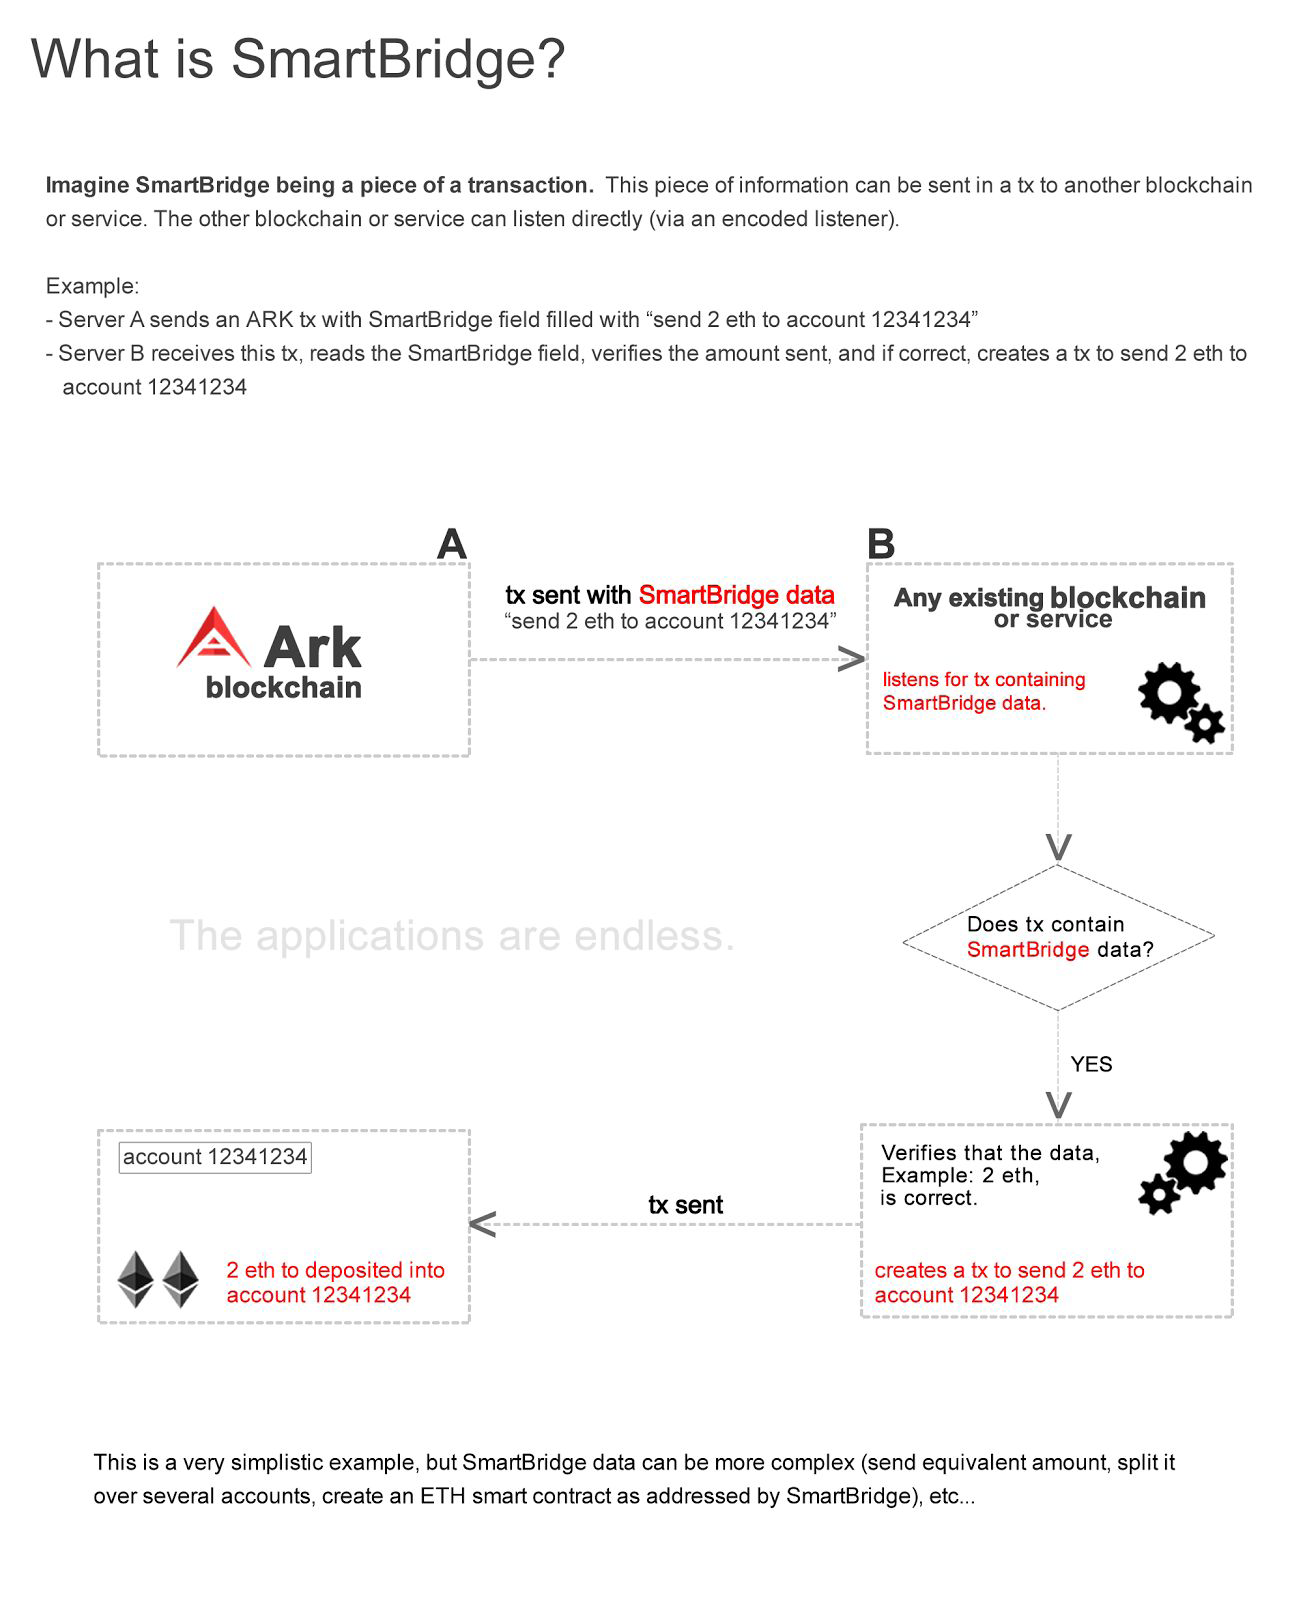
\includegraphics[width=\textwidth,height=\textheight,keepaspectratio]{ARKSmartBridge}
	\captionof{figure}{ARK SmartBridge Technology}
\end{center}

\subsection{A.C.E.S. - ARK Contract Execution Service}
ACES is a blockchain interoperability platform that provides simple protocols and tools for building a robust blockchain 
service marketplace.

ACES is composed mainly of the following three components:
\begin{description}
	\item[Listeners] ACES Listeners provide a way for all the different blockchain transaction events to be easily 
	consumed via a common REST-ful API. The API allows consumers to create subscriptions and receive blockchain events 
	in real-time using Webhook callbacks.
	\item[Services] ACES Services create and excute Service Contracts, which can be anything from uploading 
	a file to a storage blockchain, performing value transfers, creating smart contracts, executing code on 
	blockchain based computing platforms, or interacting with IoT hardware.
	\item[Marketplace Console] The ACES Marketplace Console is a consumer dashboard for searching and executing 
	service contracts listed on the Marketplace. ACES Service providers can list their service nodes using the Marketplace API.
\end{description}

\begin{center}
	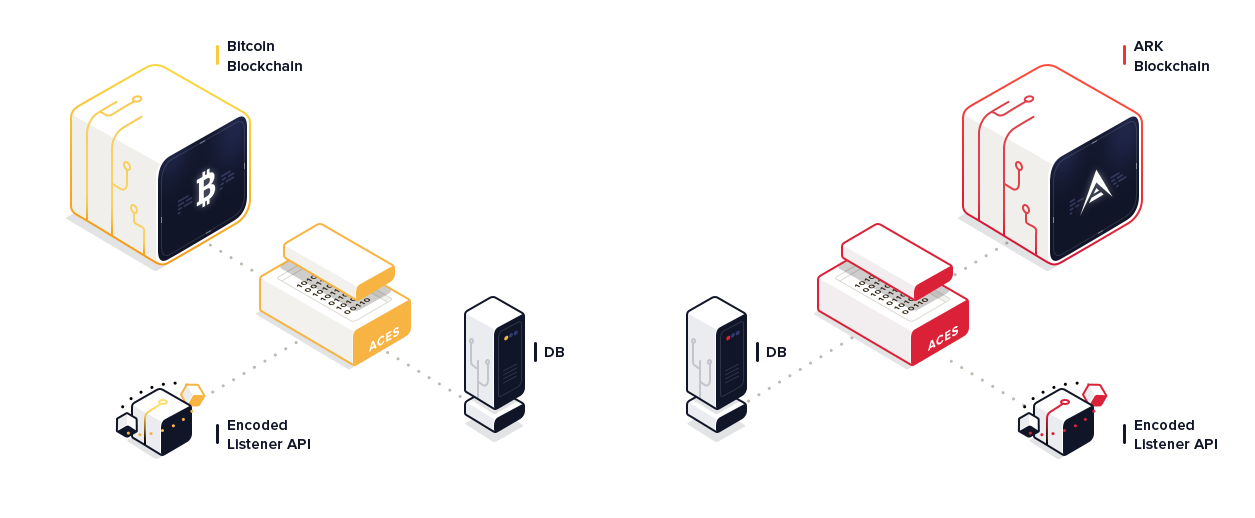
\includegraphics[width=\textwidth,height=\textheight,keepaspectratio]{ACES}
	\captionof{figure}{ARK-BTC A.C.E.S. SmartBridge Implementation Overview}
\end{center}

\section{Ripa Liquidity Service Provider (R.L.S.P)}
Using the SmartBridge technology RipaEx will build a mechanism to share liquidity between all the exchanges in the Ripa network
by writing the single exchange orderbook in the Ripa Blockchain and by executing order matching between all exchanges in the network.

In this way you can have the benefits of a decentralized orderbook (like liquidity) with the benefits of a centralized exchange (like
platinum customer support and FIAT exchange).

\section{Ripa Community Fund}
To permits the born of new exchanges in the Ripa network a Ripa Community Fund - RCF - is created with the following characteristics:
\begin{description}
	\item[Starting Principal]: the RCF will have a starting operating capital of 5\% (5,750,000 \PHP) of the genesis block
	\item[Recurring Participation]: each delegate will contribute to the RCF with 5\% of its forged XPXs
\end{description}

To obtain funds from the RCF to start your own Ripa Exchange you will submit your proposal in the official RCF section in the Ripa forum at
anytime after the first Ripa Exchange instance will be operative.

%----------------------------------------------------------------------------------------
%	CHAPTER 5: Token Sale
%----------------------------------------------------------------------------------------

\chapterimage{chapter_head_5_Tokyo.jpg} % Chapter heading image
\chapter{Token Sale}
\section{Introduction}
The RipaEx XPX token sale will be separated into two phases:
	\begin{description}
		\item[\textsc{PreSale}]: that will run from April to September 2018
		\item[\textsc{RIPA TEC}]: that will run from October to December 2018
	\end{description}

You can easily refer to both phases presale and RIPA TEC as \textit{RipaEx ICO}.

\subsection{Exchange Rate \& Accepted Cryptocurrencies}
During the token sale the exchange rate for the XPX tokens will be \textbf{\PHP/\euro0.10}.\\

The following cryptocurrencies are accepted: \textbf{BTC, ETH, ARK, LISK}.\\

If you want to send us a different cryptocurrency send us your choice and we will tell you immediately if we can make 
the exchange and how to execute the operation in detail (receiving address, exchange rate, quantity)\\

\textsc{Exchange rate is Bitstamp last and is valid 60 minutes from quote}.

\section{How to Invest}
\subsection{XPX Ripa Token PreSale}
Private sale of XPX tokens has \textbf{started on Monday 04/02/2018 at 00:00 GMT and will end on Sunday 09/30/2018 at 23:59 GMT}.

You can buy directly here: 
\begin{center}
	\href{https://www.ripaex.io/privsale}{\textsc{www.ripaex.io/privsale}}
\end{center}

or send us your buying enquiries on our social Slack, Telegram, Facebook, Twitter or on other social networks where we are present.
For all the duration of the private sale period every exchange operation \textbf{will receive a 100\% bonus on its sending amount
until the first 5.000.000 XPX tokens} have been exchanged and will receive a 50\% bonus thereafter.

\subsection{RIPA TEC}
Fundraising through the RIPA TEC platform will follow the schedule:
\begin{description}
	\item[from 10/01/2018 00:00 to 10/14/2018 23:59]: with bonus of 50\% 
	\item[from 10/15/2018 00:00 to 10/28/2018 23:59]: with bonus of 40\% 
	\item[from 10/29/2018 00:00 to 11/11/2018 23:59]: with bonus of 30\% 
	\item[from 11/12/2018 00:00 to 11/25/2018 23:59]: with bonus of 20\% 
	\item[from 11/26/2018 00:00 to 12/09/2018 23:59]: with bonus of 10\% 
	\item[from 12/10/2018 00:00 to 12/23/2018 23:59]: with bonus of 5\% 
\end{description}
Coins distribution will be available at the end of each trading day and performed automatically through the RIPA TEC platform. Minimum
threshold to reach is 25 BTC.\\

\textsc{As the XPX exchange rate is calculated against the euro currency directly you are guaranteed to not loose any invested fund
during the sale period as the XPX tokens will be listed on our exchanges at the beginning of 2019 directly with the same \textbf{\PHP/\euro0.10}
exchange rate agreed during the token sale-ICO phase}.\\

RIPA TEC platform will be available at the following link after September 2018:
\begin{center}
	\href{https://tex.ripaex.io}{\textsc{tec.ripaex.io}}
\end{center}
follow us on Facebook, Twitter, Telegram, Slack and all of our official social channel to know when RIPA TEC is starting!!

\section{XPX Ripa Token Distribution}
\textbf{115,000,000} XPX tokens are seeded into the genesis block: distribution of the XPX tokens generated are described into
figure \ref{fig:distribution} and table \ref{tab:distribution}.

\vspace{5mm}
%\begin{center}
	\begin{tikzpicture}
		\pie [rotate = 180, explode={0.2, 0.1, 0.1, 0.1, 0.1, 0.1}, radius = 3]
		{65/PreSale \& RIPA TEC,
		15/RIPA Founders Team, 
		6/for marketing,
		5/for bounties,
		5/for RCF,
		4/ARK Team}
	\end{tikzpicture}
	\captionof{figure}{Ripa token distribution - Division of funds}	
	\label{fig:distribution}
%\end{center}

\vspace{5mm}
\begin{table}[H]
	\centering
	\begin{tabular}{l l l}
		\toprule
		\textbf{Percentage (\%)} & \textbf{Quantity (\PHP)} & \textbf{Purpose} \\
		\midrule
		65		& 74,750,000	& to distribute in PreSale and RIPA TEC	\\
		15      & 17,250,000	& to the RIPA Founders Team	\\
		6       & 6,900,000		& for marketing	\\
		5       & 5,750,000 	& for bounties	\\
		5       & 5,750,000		& for Ripa Community Fund - RCF	\\
		4       & 4,600,000		& to the ARK Team	\\
		\bottomrule
	\end{tabular}
	\captionof{table}{Ripa token distribution}
	\label{tab:distribution}
\end{table}

\vspace{5mm}
\textbf{Tokens not sold during the phases of PreSale and RIPA TEC will be burnt} forever to permits and equal distributions 
of the funds and avoid speculations on the token remaining.

\section{Division of Funds}
The funds collected during the PreSale and RIPA TEC phases will be divided as explained in figure \ref{fig:division} and 
table \ref{tab:division} below

\vspace{5mm}
\begin{tikzpicture}
	\pie [rotate = 180, explode={0.2, 0.1, 0.1}, radius = 3]
	{60/for project development,
	20/for marketing, 
	20/for legal support}
\end{tikzpicture}
\captionof{figure}{Ripa division of funds}	
\label{fig:division}

\vspace{5mm}
\begin{table}[H]
	\centering
	\begin{tabular}{l l}
		\toprule
		\textbf{Percentage (\%)} & \textbf{Purpose} \\
		\midrule
		60		& for project development	\\
		20		& for marketing	\\
		20		& for legal support	\\
		\bottomrule
	\end{tabular}
	\captionof{table}{Division of funds}
	\label{tab:division}
\end{table}

\vspace{5mm}
where the row project development funds allocation is described in table \ref{tab:focus} below.

\vspace{5mm}
\begin{table}[H]
	\centering
	\begin{tabular}{l l}
		\toprule
		\textbf{Percentage (\%)} & \textbf{Purpose} \\
		\midrule
		50		& functional analysis, technical analysis, development, testing	\\
		20		& technical support	\\
		15		& infrastructure	\\
		10		& security	\\
		5		& analytics	\\
		\bottomrule
	\end{tabular}
	\captionof{table}{Project development focus}
	\label{tab:focus}
\end{table}

%----------------------------------------------------------------------------------------
%	CHAPTER 6: Economic Projections
%----------------------------------------------------------------------------------------

\chapterimage{chapter_head_6_Frankfurt.jpg} % Chapter heading image

\chapter{Business Model}

\section{Project Milestones}
Following the matrix of development per area of interest based on the funds collected during the phases of PreSale and RIPA TEC:\\
\begin{tcbraster}[raster columns=5,raster rows=1,raster height=0.8cm,
	valign=center, halign=center,
	enhanced,size=small,sharp corners,colframe=azure(colorwheel),coltext=white,
	colback=azure(colorwheel),fit algorithm=hybrid* ]
	\tcboxfit{}
	\tcboxfit{\textbf{25 BTC}}
	\tcboxfit{\textbf{250 BTC}}
	\tcboxfit{\textbf{1000 BTC}}
	\tcboxfit{\textbf{2000 BTC}}
\end{tcbraster}
\begin{tcbraster}[raster columns=5,raster rows=4,raster height=10cm,
	valign=center, halign=center,
	enhanced,size=small,sharp corners,colframe=silver,coltext=black,
	colback=silver,fit algorithm=hybrid* ]
	\tcboxfit{\textsc{\textbf{Development}}}
	\tcboxfit{\tcbfontsize{0.8} CRYPTO <-> CRYPTO exchange release with 25 cryptocurrencies supported and 3 main trading pairs}
	\tcboxfit{\tcbfontsize{0.8} CRYPTO <-> FIAT exchange release with MasterCard prepaid card. 50 cryptocurrencies supported and 3 main trading pairs}
	\tcboxfit{\tcbfontsize{0.8} Advanced trading features. Open of a second and third Ripa Exchanges to join the Ripa network}
	\tcboxfit{\tcbfontsize{0.8} Open of ten Ripa Exchanges across the Globe}

	\tcboxfit{\textsc{\textbf{Marketing}}}
	\tcboxfit{\tcbfontsize{0.8} Support from one agency, adv campaigns on targeted channels}
	\tcboxfit{\tcbfontsize{0.8} Support from three agencies, adv capaigns pushing harder, store with RipaEx gadgets}
	\tcboxfit{\tcbfontsize{0.8} International presentation event in London}
	\tcboxfit{\tcbfontsize{0.8} Support from five agencies, targeting all UN countries, presentation event in Tokyo}

	\tcboxfit{\textsc{\textbf{Legal}}}
	\tcboxfit{\tcbfontsize{0.8} Legal department working on AML/KYC international standards}
	\tcboxfit{\tcbfontsize{0.8} Legal departments working on AML/KYC international standards in New York, London, Hong Kong}
	\tcboxfit{\tcbfontsize{0.8} International Government Agencies cooperation}
	\tcboxfit{\tcbfontsize{0.8} Banking parnership for defining AML/KYC standards}

	\tcboxfit{\textsc{\textbf{Blockchain}}}
	\tcboxfit{\tcbfontsize{0.8} DevNET development for RLSP and future ARK releases}
	\tcboxfit{\tcbfontsize{0.8} Contributions to ARK development for AVM}
	\tcboxfit{\tcbfontsize{0.8} Contributions to ARK development for standard timing releases}
	\tcboxfit{\tcbfontsize{0.8} Partnership with ARK for blockchain technology developments}
\end{tcbraster}

\section{Market Overview}

\section{Local Market Analysis}

\section{5 Years Projections}

\section{XPX Token Economics}

%----------------------------------------------------------------------------------------
%	CHAPTER 7: Conclusion
%----------------------------------------------------------------------------------------

\chapterimage{chapter_head_7_LosAngeles.jpg} % Chapter heading image

\chapter{Team \& Conclusion}

\section{Team}
\begin{tcbraster}[raster columns=1,raster rows=1,raster height=0.4cm,
	valign=center, halign=center,
	enhanced,size=small,sharp corners,colframe=azure(colorwheel),coltext=white,
	colback=azure(colorwheel),fit algorithm=hybrid* ]
	\tcboxfit{}
\end{tcbraster}
\begin{tcbraster}[raster columns=2,raster rows=4,raster height=10cm,
	valign=center, halign=left,
	enhanced,size=small,sharp corners,colframe=silver,coltext=black,
	colback=silver,fit algorithm=hybrid* ]
	\tcboxfit{\tcbfontsize{0.8} \textbf{Giovanni Silvestri @ BitNow}\\
	\textsc{CEO, founder and head of the project}\\
	10+ years experience in IT field,\\
	4+ years in cryptocurrencies consultancy and exchanging,\\
	2+ years experience in finance,\\
	Location: Treviso (TV), Italy\\
	\href{https://bitcointalk.org/index.php?action=profile;u=497151;sa=summary}{\faBitcoin}
	\href{https://www.linkedin.com/in/zackko/}{\faLinkedin}}
	\tcboxfit{\tcbfontsize{0.8} \textbf{Antonello Arena}\\
	\textsc{CFO}\\
	10+ years experience in economics and finance,\\
	4+ years in cryptocurrencies consultancy and exchanging,\\
	Location: Potenza (PO), Italy\\
	\href{https://www.linkedin.com/in/antonello-arena-a26b60b7/}{\faLinkedin}}

	\tcboxfit{\tcbfontsize{0.8} \textbf{Giorgio Isola @ilgio}\\
	\textsc{CDO}\\
	10+ years experience in design,\\
	4+ years in cryptocurrencies consultancy and exchanging,\\
	Location: Milan (MI), Italy\\
	\href{https://bitcointalk.org/}{\faBitcoin}
	\href{https://www.linkedin.com/}{\faLinkedin}}
	\tcboxfit{\tcbfontsize{0.8} \textbf{Your Name Here}\\
	\textsc{CSO}\\
	5+ years experience in IT networking,\\
	2+ years in network security,\\
	2+ years experience in finance and or cryptocurrencies,\\
	Location: \\
	\href{https://bitcointalk.org/}{\faBitcoin}
	\href{https://www.linkedin.com/}{\faLinkedin}}

	\tcboxfit{\tcbfontsize{0.8} \textbf{Your Name Here}\\
	\textsc{developer}\\
	3+ years experience in programming,\\
	1+ years in Ruby on Rails,\\
	Nice to have 1+ years experience in finance and or cryptocurrencies,\\
	Location: \\
	\href{https://bitcointalk.org/}{\faBitcoin}
	\href{https://www.linkedin.com/}{\faLinkedin}}
	\tcboxfit{\tcbfontsize{0.8} \textbf{Your Name Here}\\
	\textsc{developer}\\
	3+ years experience in programming,\\
	1+ years in Ruby on Rails,\\
	Nice to have 1+ years experience in finance and or cryptocurrencies,\\
	Location: \\
	\href{https://bitcointalk.org/}{\faBitcoin}
	\href{https://www.linkedin.com/}{\faLinkedin}}

	\tcboxfit{\tcbfontsize{0.8} \textbf{Your Name Here}\\
	\textsc{Technical support}\\
	3+ years experience in Front-End office support,\\
	Nice to have 1+ years experience in finance and or cryptocurrencies,\\
	Location: \\
	\href{https://bitcointalk.org/}{\faBitcoin}
	\href{https://www.linkedin.com/}{\faLinkedin}}
	\tcboxfit{\tcbfontsize{0.8} \textbf{Your Name Here}\\
	\textsc{Technical support}\\
	3+ years experience in Front-End office support,\\
	Nice to have 1+ years experience in finance and or cryptocurrencies,\\
	Location: \\
	\href{https://bitcointalk.org/}{\faBitcoin}
	\href{https://www.linkedin.com/}{\faLinkedin}}

	\tcboxfit{\tcbfontsize{0.8} \textbf{Your Name Here}\\
	\textsc{community manager America}\\
	3+ years experience in moderating community,\\
	1+ years in finance and or cryptocurrencies,\\
	Location: \\
	\href{https://bitcointalk.org/}{\faBitcoin}
	\href{https://www.linkedin.com/}{\faLinkedin}}
	\tcboxfit{\tcbfontsize{0.8} \textbf{Your Name Here}\\
	\textsc{community manager EMEA}\\
	3+ years experience in moderating community,\\
	1+ years in finance and or cryptocurrencies,\\
	Location: \\
	\href{https://bitcointalk.org/}{\faBitcoin}
	\href{https://www.linkedin.com/}{\faLinkedin}}

	\tcboxfit{\tcbfontsize{0.8} \textbf{Your Name Here}\\
	\textsc{community manager Africa}\\
	3+ years experience in moderating community,\\
	1+ years in finance and or cryptocurrencies,\\
	Location: \\
	\href{https://bitcointalk.org/}{\faBitcoin}
	\href{https://www.linkedin.com/}{\faLinkedin}}
	\tcboxfit{\tcbfontsize{0.8} \textbf{Your Name Here}\\
	\textsc{community manager Asia}\\
	3+ years experience in moderating community,\\
	1+ years in finance and or cryptocurrencies,\\
	Location: \\
	\href{https://bitcointalk.org/}{\faBitcoin}
	\href{https://www.linkedin.com/}{\faLinkedin}}

	\tcboxfit{\tcbfontsize{0.8} \textbf{Your Name Here}\\
	\textsc{Delegate}\\
	3+ years experience in DPOS delegation,\\
	1+ years in finance and or cryptocurrencies,\\
	Location: \\
	\href{https://bitcointalk.org/}{\faBitcoin}
	\href{https://www.linkedin.com/}{\faLinkedin}}
	\tcboxfit{\tcbfontsize{0.8} \textbf{Your Name Here}\\
	\textsc{Delegate}\\
	3+ years experience in DPOS delegation,\\
	1+ years in finance and or cryptocurrencies,\\
	Location: \\
	\href{https://bitcointalk.org/}{\faBitcoin}
	\href{https://www.linkedin.com/}{\faLinkedin}}

	\tcboxfit{\tcbfontsize{0.8} \textbf{Your Name Here}\\
	\textsc{Delegate}\\
	3+ years experience in DPOS delegation,\\
	1+ years in finance and or cryptocurrencies,\\
	Location: \\
	\href{https://bitcointalk.org/}{\faBitcoin}
	\href{https://www.linkedin.com/}{\faLinkedin}}
	\tcboxfit{\tcbfontsize{0.8} \textbf{Your Name Here}\\
	\textsc{Delegate}\\
	3+ years experience in DPOS delegation,\\
	1+ years in finance and or cryptocurrencies,\\
	Location: \\
	\href{https://bitcointalk.org/}{\faBitcoin}
	\href{https://www.linkedin.com/}{\faLinkedin}}
\end{tcbraster}

\section{Recommendations}
If you are planning to start your own crypto asset marketplace you are invited to follow the following procedure to make
your start-up plan a success in the Ripa ecosystem:
\begin{enumerate}
	\item Submit your proposal to Ripa Community Fund by its official website\footnote{available after March 2019} or by contacting us
	on our official social channels
	\item Get the funds you need from RCF, Venture Capital or ICO
	\item Decide the functional specifications of your exchange
	\item Implement the exchange
	\item Open to public
\end{enumerate}

Following the procedure above you are guaranteed to start a successful exchange for which you own the source code and which will 
generate revenues for your business action in the 5 years timespan.

It can't be enough stressed out that if your intent is to open a FIAT <-> CRYPTO exchange you should
focus from the first instance on law compliance by studying the AML/KYC laws of the country of incorporation and
finding bank partners to work with. Local financial Authority can help to comply with rules \& regulations and 
local cryptocurrencies foundations can help you to tune your exchanges operations to perform targeted
operations based on the customers interests in the country of incorporation. 
Promote cryptocurrency-friendly users in the area of interest.\\

Remember that \textbf{\textsc{running an exchange is hard}} but we'll give you all the tools to start your adventure with all you need:
source code, liquidity and financing will be available to you from day 1 of your trading operations so you can focus on giving
platinum customer support, law compliance and partnering with financial institutions for the success of your entrepreneurship action.

\textsc{Your success is the success of the ripa exchange network} and we want to achieve that with hard work and the most advanced
technology in the industry for \textsc{YOU} and for the satisfaction of the ripa networks clients.

\section{Social}

%----------------------------------------------------------------------------------------
%	CHAPTER 8: Legal
%----------------------------------------------------------------------------------------

\chapterimage{chapter_head_8_KualaLumpur.jpg} % Chapter heading image

\chapter{\textsc{Legal}}
\begin{scriptsize}
	{\scshape
		\section{\textsc{Premise}}
		Please read this section carefully; if you have any doubts,
		please consult with your trusted legal advisor.
		\section{\textsc{Statute of liability}} 
		The RipaEx White Paper was approved by the majority of Ripa Founder Team.
		The directors and members of the TEC executive and
		management team accept full responsibility deriving
		from the statements in the white paper and ensure, in
		good faith, that what is written does not contain false
		information or omissions that could compromise the
		project’s successful outcome or the actual advantage that
		SUPPORTERS might have in any way if they decide to be
		part of the project.
		\section{\textsc{Important Information}}
		\begin{enumerate}
			\item The RipaEx and its XPX Coins are not intended to constitute
			a security in any jurisdiction.
			This White Paper regarding the TEC does not constitute
			and is not intended as a prospect or proposes itself
			as a document of any legal value in any state, and does
			not intend to constitute a securities offering or a
			solicitation for investment in securities in any jurisdiction.
			\item This White Paper is not, and should not be interpreted as a
			recommendation from the creators themselves for investing
			in the project. This WhitePaper does not replace, and
			should not be considered an independent analysis or commercial
			evaluation. Each recipient of the White Paper itself
			should have carried out market surveys and evaluations
			and have carefully considered the investment in terms of
			risks, personal possibilities and any complications in his or
			her economic potential as a result of the investment itself.
			\item The distribution of documents related to the White Paper,
			the Overview and any other information regarding this TEC
			may be prohibited by the laws of your state or jurisdiction.
			Anyone who wishes to distribute documents relating to this 
			TEC must independently ascertain, through their
			advisers, the legitimacy of such documents’ distribution
			in their country of residence or domicile. RipaEx declines
			any responsibility for the distribution of its produced
			documents in states where such distribution is restricted
			or prohibited.
			\item No person is held, invited or required to enter into any
			commercial, legal or investment contract with respect to
			the RIPA TEC or future investments in the project itself.
			\item With regard to the purchase and sale of Coins deriving
			from the investments obtained by the TEC, each user will
			have full marketing and exchange freedom of the same by
			means of private exchange or buyer who is available for
			the same and has the legal ability to purchase such Coins
			in his/her state.
			\item No legal authority has examined or approved these documents,
			which have been written using as an example the
			laws governing the publication of texts and documents in
			Europe at the time of publication. Such documents may
			not be approved or comply with the laws of SUPPORTERS’
			states, in which case a lawyer should be consulted for
			further information regarding the structured rules of this
			TEC and the international laws to which it will be submitted
			once it is launched.
			\item The risks associated with investments, the value of Coins
			and the finalization of the project will be appropriately
			clarified in the “Risks” section of this document.
			\item Reproduction, modification or dissemination of this
			document for commercial or criminal purposes is strictly
			forbidden.
			\item Accepting delivery of this White Paper (which is considered
			as its download, access to the Website: https://ripaex.io or 
			in any way accessing this White Paper), each recipient
			accepts the terms with which this White Paper is provided.
			The recipient also agrees and confirms that:
			\begin{description}
			\item[A)] he or she will keep all this information and data confidential;
			\item[B)] he or she has received this Document and/or purchased
			the XPX Coins legitimately in all jurisdictions to
			which the recipient is subject;
			\item[C)] he or she complies with all the applicable laws in relation
			to the respect of this White Paper and the purchase
			of the XPX Coins themselves.;
			\item[D)] Executors and their respective directors, officials,
			employees and professional advisers are not and will
			not be in breach of the laws of a jurisdiction to which the
			recipient is subject following the delivery of the White
			Paper and/or the purchase of XPX and will not have any
			liability in the event that such delivery of the White Paper
			or the purchase of XPX is or becomes illegal, inapplicable,
			voidable or cancelled;
			\item[E)] is aware that the XPX Coins will be offered, sold,
			transferred or otherwise disposed of directly or indirectly
			in accordance with relative sales restrictions and all applicable
			laws;
			\item[F)] has sufficient knowledge and experience in financial
			and commercial matters to be able to assess the merits
			and risks of purchasing XPX Coins and is able and willing
			to withstand the economic and financial risks of purchasing
			and/or holding the XPX Coins themselves.
			\item[G)] acquires XPX on his or her own account and not for
			third parties;
			\item[H)] accepts and acknowledges that Coins issued by RipaEx
			must not be interpreted, classified or treated as:
			(I) any type of currency other than current cryptocurrencies;
			(Ii) bonds, shares or shares issued by any person or entity;
			(Iii) rights, options or derivative instruments relating to
			such bonds or shares;
			(Iv) the rights to secure a profit or to avoid a loss;
			(V) units in any type of investment scheme;
			(Vi) units in any type of trust;
			(Vii) any form of derivative;
			(Viii) any other guarantee or class of securities.
			\item[I)] is aware that the information contained in this White
			Paper may not be complete or may be modified later.
			\item[J)] is fully informed and aware of all matters relating to the
			purchase, sale and holding of XPX in any form whatsoever
			which cannot be specifically indicated in this Overview or
			White Paper document, but which may be disclosed to a person 
			who can reasonably be inferred to have the knowledge
			and familiarity with the problems and complications
			of Cryptocurrencies such as Bitcoins, Ethereum and/or
			other types of cryptokens and confirms in an irrevocable
			and unconditional manner that he or she has an understanding
			of the operation, functionality, usage, storage,
			transmission mechanisms and other material features of
			Cryptocurrencies, blockchain-based software systems,
			cryptocurrency wallets and smart contract technology.
			\end{description}
			\item This document may include certain historical information,
			estimates or reports arising from sources cited in this
			document or others related to the TEC, material activities
			carried out by the program’s executors and other issues.
			No statement or guarantee is provided regarding the accuracy
			or completeness of any information, estimate and/
			or reporting of any such information or other third party
			sources.
			\item The document includes “forward-looking statements”.
			These statements include, among other things, the
			discussions of each of RipaEx’s business strategies and
			expectations regarding its position in the economy, future
			operations, profitability, liquidity, assets and financial
			position. All of these statements are based on estimates
			and assumptions made by the program’s executors who,
			although considered reasonable, are subject to risks and
			uncertainties that may cause real events and that the
			results of the programs’ executors are materially different
			from those anticipated or indicated by such declarations
			and estimates and no guarantees may be given that any
			such statements or estimates will be made. In the light of
			these and other uncertainties, the inclusion of a forwardlooking
			statement in this document or the White Paper
			itself should not be considered as a representation or a
			guarantee by the TEC in any case.
			\item This document and its contents are strictly confidential
			and the information contained herein is provided to the recipient
			strictly based on the fact that the recipient ensures
			that such information is confidential.
			Consequently, this document and its contents or any
			information made available to the recipient in connection
			with further investigations must be securely kept. In the
			event of a breach of this confidentiality guarantee or if it is 
			reasonably likely that such confidentiality may be infringed
			on, the Program Authors may, at their discretion, request
			any remedy available to the program executors, whether
			under the law or based on net equity for damages. The
			executor programs’ have the right to completely recover all
			the costs, expenses and losses incurred and/or suffered
			in this regard from the criminal subject. To eliminate any
			doubt, this confidentiality is held as attributable to the
			recipient, professional advisers, administrators, employees
			and other persons affected by the program, as well as executors
			or any other person to which the plans and goals
			of the program executors will reach.
			\item RipaEx does not guarantee and does not undertake to
			provide any returns to its participants. All that is written in
			the White Paper is based on industry studies and analyses
			carried out by professionals and technicians, which could
			be inaccurate or conclude with a negative outcome.
			The value of XPX Coins is absolutely uncertain and not
			guaranteed.
			The buyback commitment will be respected within the
			terms defined in this document.
			\item RipaEx guarantees all its commitment and physical and mental
			effort to complete the project in the times described
			and appropriately detailed in this document, however,
			it does not assume responsibility for project delays or
			delays due to third party events, legal, administrative or
			catastrophic events that could lead to an interruption in
			the project itself.
			\item The risks section is organized to incorporate, along with
			these legal disclaimers, a type of warning to SUPPORTERS
			about the possible losses of an investment on a type of
			investment such as an TEC.
		\end{enumerate}		
	}
\end{scriptsize}
%----------------------------------------------------------------------------------------
%	BIBLIOGRAPHY
%----------------------------------------------------------------------------------------

\chapterimage{chapter_head_9_Milan.jpg} % Chapter heading image

\addcontentsline{toc}{chapter}{\textcolor{trolleygrey}{References}}
\nocite{*}
\printbibliography[title={References}]
%------------------------------------------------


%----------------------------------------------------------------------------------------
%	COPYRIGHT PAGE
%----------------------------------------------------------------------------------------

\newpage
~\vfill
\thispagestyle{empty}

\noindent Copyright \copyright\ 2018 Ripa Founder Team\\ % Copyright notice

\noindent \textsc{Published by Ripa Founder Team}\\ % Publisher

\noindent \textsc{www.ripaex.io}\\ % URL

\noindent Licensed under the MIT License (the ``License''). You may not use this file except in compliance with the License. You may obtain a copy of the License at \url{https://opensource.org/licenses/MIT}. Unless required by applicable law or agreed to in writing, software distributed under the License is distributed on an \textsc{``as is'' basis, without warranties or conditions of any kind}, either express or implied. See the License for the specific language governing permissions and limitations under the License.\\ % License information

\noindent \textit{First printing, March 2018} % Printing/edition date

\end{document}
